\documentclass[11pt, preprint, twoside]{aastex}
\usepackage{epsfig}
\usepackage{rotating}
\usepackage{makecell}


% ISSUES:
%  Spring/Fall -- no "Spring" version of Starry Night indoor lab

% EACH YEAR:
%  remind Salvati about first lab being first week
%  update final exam time

%  interesting events
%  redo planet locations in Lab #1 
%  redo weekly outlook in syllabus
%  update office hours in syllabus
%  update TA information in syllabus
%  update class times in syllabus 



\renewcommand{\u}{\ensuremath{u}}
\newcommand{\g}{\ensuremath{g}}
\renewcommand{\r}{\ensuremath{r}}
\renewcommand{\i}{\ensuremath{i}}
\newcommand{\z}{\ensuremath{z}}

\newcommand{\kms}{\hbox{km\,s$^{\rm -1}$}}
%\def\kms{\ifmmode {\,{\rm km\,s^{-1}}}                          % km s-1
%        \else {\hbox{$\,$ {\rm km$\,$s$^{\rm -1}$}}}\fi}
%\def\solar {\ifmmode_{\mathord\odot} \else $_{\mathord\odot}$\fi} % _solar
%\def\mo {\ifmmode {\,{\it M}\solar} \else $\,M$\solar\fi}       % M solar
\def\lo {\ifmmode {\,{\it L}\solar} \else $\,L$\solar\fi}       % L solar
\def\my {\ifmmode {\,{\it M}\solar\,{\rm yr^{-1}}}              % Msol/year
        \else {$\,M$\solar$\,$yr$^{\rm -1}$}\fi}
\def\BD {BD$\,$+30{\degr}3639}
\def\HUNO{\rm H$\,$I}                   % molecular hydrogen
\def\HDOS{\rm H$_2$}                    % molecular hydrogen
\def\arcsec{\ifmmode {^{\scriptscriptstyle\prime\prime}}
          \else $^{\scriptscriptstyle\prime\prime}$\fi}
\def\arcminm{\ifmmode {^{\scriptscriptstyle\prime}}
          \else $^{\scriptscriptstyle\prime}$\fi}
\def\deg{\ensuremath{^\circ}}


\newcounter{thelabs}
\newcommand{\labnum}{\arabic{thelabs}}

\newcounter{thelecs}
\newcommand{\lecnum}{\arabic{thelecs}}

\begin{document}

\noindent{\bf Observational Astronomy / PHYS-UA 13 / Fall 2022 /
  Syllabus }

\noindent {\bf Course Summary}: This course will teach you how to
observe the sky carefully with your naked eye, binoculars, and a small
telescope. You will learn the basics of observable lunar and planetary
properties, and the basics of astronomical coordinates and
observations. The goal is for you to be able to understand and
describe what you see in the sky at night, and to be able to use
charts and coordinates to predict it.

\noindent {\bf Instructors}: Prof. Michael Blanton (726 Broadway,
Rm 941, {\tt mb144@nyu.edu}) and TA Nick Faucher ({\tt
  ntf229@nyu.edu}).

\noindent {\bf Help \& Questions Time}: Prof. Blanton will be available in
  his office and/or on Zoom every Wednesday from 12:30pm to 2pm if you
  have questions or need help with the classwork. Feel free to email
  with an alternative appointment time if that time does not work.
 
\noindent {\bf Books}: The primary books are below.
\begin{itemize}
\item {\it Astronomy: A Self-Teaching Guide}, by Dinah Moche
\item {\it The Amateur Astronomer's Introduction to the Celestial
  Sphere}, by William Millar
\item This laboratory manual. 
\end{itemize}
There is a digital reserve copy of Moche available at the NYU
Library. For Millar, as of writing this syllabus, it is not
available through the library. This lab manual is available in PDF
format on Brightspace. We will also use the following books:
\begin{itemize}
\item {\it Sky \& Telescope's Pocket Sky Atlas}, by Roger W.~Sinnott
(we have copies in the lab rooms).
\item {\it Edmund Mag 5 Star Atlas} (will be supplied to you)
\end{itemize}

\noindent {\bf Lecture}: Each week you will attend one lecture
(at 3:30pm Monday in Room 369 of the Global Center of Academic \&
Spiritual Life). There is reading material listed for each week, and I
will distribute notes on Brightspace prior to each lecture too; it
will be best to read that material {\it before class}.  There will be
quizzes every lecture that will contribute to your grade, and other
activities that you will also learn from, so please attend! Let me
know {\it ahead of time} if you cannot.

\noindent {\bf Grading}: Grades are based on labs (20\% on written
material, 5\% on extra good work), weekly lecture questions (25\%),
weekly quizzes (10\%), one midterm (20\%), and the final (20\%).

\noindent {\bf Lecture Questions}: Each week (starting with the second week)
you will hand in the lecture questions associated with the previous
weeks' lecture. I will grade two of the questions each week (I won't
tell you which!).

\noindent {\bf Quizzes}: Each week (starting with the second week)
there will be a 5-minute quiz at the start of lecture.  Questions will
be based on the lecture questions due that day, and will involve the
conceptual questions (i.e. I won't ask the exact mass of the Sun or
other pure memorization questions).  Prepare for the quiz by answering
the lecture questions each week! For the quiz itself, I'll present two
question options and you can answer either one of the two questions.

\noindent {\bf Exams}: For the midterm and the final you are
responsible for material in the labs, the reading, and the
homework. In preparing for the exams, use the lecture question as a
guide to which material I believe is essential and the types of
questions I will ask.

\noindent {\bf Lab (meet in Meyer 224)}: Arrive on time at 7:00pm for
the lab. We will discuss the contents of the lab and conduct some
indoor activities. If weather permits, we will proceed to the rooftop
observatory. If weather doesn't permit, we will have indoor
activities.

\noindent {\bf What If I Have to Miss Lab?}: If you must miss lab due
to medical reasons or a truly unavoidance circumstance, contact the
professor {\it and} the TA with the justification. Other than such
circumstances, you can miss {\bf one lab} during the semester without
penalty: you must however contact the lab instructor explicitly {\bf
beforehand} to claim this credit. If you are absent for any other lab
without good cause you will lose credit for that lab.  If you miss
more than three labs without good cause, you will not be given a
passing grade in the course.

\noindent {\bf Weekly Lab Entries}: Finally, the last lab in this book
should have entries filled in {\bf every week}, and should be handed
in on the final lab date.

\noindent {\bf No Switching Between Labs}: You cannot switch
between the lab's Monday and Wednesday sections mid-semester, because
in general they will be on different schedules. The timing of the
indoor and outdoor labs for each section will be driven mostly by the
weather. 

\noindent {\bf Dress Warmly}: Please dress appropriately for remaining
outside for an extended period, including hats and gloves when
appropriate, which will be more often than you think.

\noindent {\bf Do not use your phones during lab unless directed
to!}

\noindent {\bf Accommodations}: I am committed to creating an
inclusive and accessible classroom environment for students of all
abilities. Students who may need academic accommodations are advised
to reach out to the Moses Center for Student Accessibility as early as
possible in the semester for assistance (212-998-4980 or {\tt
mosescsd@nyu.edu}). Information about the Moses Center can be found at
{\tt \url{http://www.nyu.edu/csd}}.  If you need any support in
connecting with the Moses Center or other resources, please also let
me know. Students who need accommodations for the laboratory component
of the class should talk to me about their needs so we can arrange a
solution.

\noindent {\bf Health}: I encourage all students to
attend to their general mental and physical health. To access the
University's extensive health and mental health resources, contact the
NYU Wellness Exchange. You can call its private hotline (212-443-9999)
or chat (in six different languages) via the Wellness Exchange app or
at {\tt wellness.exchange@nyu.edu}, available 24 hours a day, seven
days a week, to reach out to a professional who can help to address
day-to-day challenges as well as other health-related concerns.

\clearpage

\baselineskip 0pt
\begin{sidewaystable}
\small
\begin{tabular}{|c||c|c|}
\hline
{\it Sep.~12} 
& The Celestial Sphere: angles \& coordinates 
& Millar Ch.~2; Edmund pp.~1--9; Moche 1.1--1.15
\cr 
{\it Sept.~19} 
& Introduction to telescopes
& Moche 2.11--2.21
\cr
{\it Sept.~26} 
& Rotation and Orbit of the Earth
& Millar Ch.~4.1--4.5, Ch.~6; Moche 1.16--1.23
\cr
{\it Oct.~3} 
& Finding your way in the sky
& Edmund pp.~30--32
\cr
{\it Oct.~11} {\bf (Tuesday!)}
& Stars
& Millar Ch.~3; Moche Ch.~3
\cr
{\it Oct.~17} 
& Variables and Binaries
& Millar Ch.~3
\cr
{\it Oct.~24} 
& {\bf Midterm exam in class!}
& ---
\cr
{\it Oct.~31} 
& Galaxies
& Moche Ch.~6
\cr
{\it Nov.~7} 
& The Moon
& Millar Ch.~6; Edmund p.~34; Moche Ch.~10
\cr
{\it Nov.~14} 
& Planets and their motions
& Moche Ch. 8.5--8.9, Ch.~9
\cr
{\it Nov.~21} 
& Moons of Jupiter and Saturn
& Moche Ch.~9
\cr
{\it Nov.~28} 
& Precession \& nutation


& Millar Ch.~4.6--4.7
\cr
{\it Dec.~5} 
& Tides \& Eclipses
& Millar Ch.~7
\cr
{\it Dec.~12} 
& Asteroids, Comets, Meteors
& Moche Ch.~11
\cr
{\it Dec. 20 2:00pm--3:50pm}
& {\bf FINAL EXAM, GCASL 369}
& 
\cr
\hline
\end{tabular}
\end{sidewaystable}

\clearpage

\baselineskip 0pt
\begin{sidewaystable}
\small
\begin{tabular}{|c|c|c|c|c|}
\hline
{\it Sept.~12--14} 
& Jupiter, Saturn
& ---
& Waxing Gibbous Moon
& Sunset 7:07pm EDT
\cr
{\it Sept.~19--21} 
& Jupiter, Saturn
& Andromeda rising
& ---
& Sunset 6:56pm EDT
\cr
{\it Sept.~26--28}
& Jupiter, Saturn
& Andromeda
& ---
& Sunset 6:44pm EDT
\cr
{\it Oct.~3--5}
& Jupiter, Saturn
& Andromeda
& First Quarter Moon
& Sunset 6:32pm EDT
\cr
{\it Oct.~11--12}
& Jupiter, Saturn
& Andromeda
& Waxing Gibbous Moon
& Sunset 6:21pm EDT
\cr
{\it Oct.~17--19}
& Jupiter, Saturn
& Andromeda
& ---
& Sunset 6:10pm EDT
\cr
{\it Oct.~24--26} 
& Jupiter, Saturn
& Andromeda
& ---
& Sunset 6:00pm EDT
\cr
{\it Oct.~31--Nov.~2}
& Jupiter, Saturn
& Andromeda
& First Quarter Moon
& Sunset 5:52pm EDT
\cr
{\it Nov.~7--9}
& Jupiter, Saturn, Mars rising
& Andromeda, Pleiades
& Full Moon
& Sunset 4:44pm EST
\cr
{\it Nov.~14--16}
& Jupiter, Saturn, Mars rising
& Andromeda, Pleiades
& ---
& Sunset 4:37pm EST
\cr
{\it Nov.~21}\footnote{No lab on Wednesday, November 23 (night before
Thanksgiving)}
& Jupiter, Saturn, Mars
& Andromeda, Pleiades
& --- 
& Sunset 4:32pm EST
\cr
{\it Nov.~28--30}
& Jupiter, Saturn, Mars
& Andromeda, Pleiades
& First Quarter Moon
& Sunset 4:29pm EST
\cr
{\it Dec.~5--7}
& Jupiter, Saturn, Mars
& Andromeda, Pleiades
& Full Moon (close to Mars on 7th)
& Sunset 4:28pm EST
\cr
{\it Dec.~12--14}
& Jupiter, Saturn, Mars
& Andromeda, Pleiades
& ---
& Sunset 4:29pm EST
\cr
\hline
\end{tabular}
\end{sidewaystable}

\clearpage

Eclipses Fall 2022:
\begin{itemize}
\item Nov. 8: Total Lunar Eclipse (maximum around 6am ET)
\end{itemize}

\baselineskip 12pt


\clearpage
%\noindent{\bf NYU City Observatory Inventory}

\noindent Telescopes
\begin{itemize}
\parskip 0pt
\parsep 0pt
\baselineskip 0pt
\item Orion (ID number, size, notes, battery needs)
\item Meade (ID number, size, notes, battery needs)
\end{itemize}

\noindent Binoculars
\begin{itemize}
\parskip 0pt
\parsep 0pt
\baselineskip 0pt
\item ID number, size, notes
\end{itemize}

\noindent Eyepieces
\begin{itemize}
\parskip 0pt
\parsep 0pt
\baselineskip 0pt
\item size, number, notes
\end{itemize}

\noindent Miscellaneous
\begin{itemize}
\parskip 0pt
\parsep 0pt
\baselineskip 0pt
\item electronic accessories
\item flashlights
\end{itemize}



\noindent{\bf Observational Astronomy / Basic observatory instructions}

\noindent For every lab, we will meet in Meyer 224, and all
go together to the roof if we are having an outdoor lab (which won't
be decided until the last minute). {\bf Be on time, otherwise we may
have left already and you will miss lab!}

\medskip \noindent On the roof, it will be cold. {\bf DRESS MUCH MORE
WARMLY THAN YOU WOULD ORDINARILY BASED ON THE WEATHER}. You will be
able to take extra clothing off if it is unnecessary, but you won't be
able to put on extra clothing you didn't bring, so err on the side of
warmth!  This isn't like skiing or hiking or even walking in the cold
--- you will be standing stock still for a couple of hours. So dress
WARMLY.

\medskip \noindent Do not leave the roof without handing in your lab
and telling an instructor.

\medskip \noindent For the labs using telescopes (all outdoor ones
except the first), we will begin lab by moving the telescopes outside.
Make sure they are evenly spaced across the roof, and that each one
has a view of Polaris to the North. If you are using an equatorial
telescope, check that the batteries to its motor are working. Make
sure to get eyepieces from the lab room. Some useful tools are also
available in the lab room: binoculars, flashlights, and some sky
atlases, for example. 

\medskip
\noindent
Below we give some basic information about the telescopes. 

\medskip
\noindent
\emph{Optics}. The telescopes for this lab have apertures of 8 to 10
inches diameter, which allows them to collect much more light than the
human eye (about 500 times more) so that we can see much fainter
objects.  The optics are quite complicated. At the front is a
transparent plate, and in the center a small secondary mirror pointing
inwards. The main optical component is a converging mirror at the
other end of the telescope. The light from a distant star passes
through the glass plate, bounces off the primary mirror, comes back up
the tube, is reflected back down the tube by the secondary and passes
through a hole in the primary mirror to the eyepiece.  There is a knob
on the back of the telescope that focuses the optics. Once set up,
this does not need to be adjusted unless you change the eyepiece.

\medskip \noindent \emph{Magnification}. When you look through the
eyepiece the view is magnified.  The magnification is given by the
formula $m = f_o/f_e$ where $f_e$ is the focal length of the eyepiece
and $f_o$ is the focal length of the objective or primary optical
component. $f_e$ is usually written on the eyepieces in mm. $f_o$ for
our telescopes is about 2500 mm. So for a 25 mm eyepiece the
magnification is 2500/25 = 100. We have a variety of eyepieces
available in the lab room. Please take these from the lab room at the
beginning of each lab and return them at the end.

\medskip \noindent \emph{Finder}. Attached to the side of the
telescope is a small finder telescope -- it acts a bit like the sights
on a rifle. It has a magnification of 6, and sees about 5\deg\ of the
sky -- much more than through the main eyepiece. When you look though
the finder there is a cross hair, that should be aligned so that a
star on the cross hair appears in the eyepiece. Thus one way to
observe a star is to line up the telescope roughly in the direction of
the star; then line up the star in the finder. It should then appear
in the main eyepiece.

\medskip \noindent \emph{Control}. The telescopes come in two
varieties.  The ``equatorial'' telescopes have two moving axes that
correspond to the sky coordinates RA and Dec. Each axis has a scale
which enables you to dial in and point at a star of known
coordinates. The Dec circle is marked in degrees; the RA circle in
hours, with smaller 5 min ticks. To move over large angles: release
the axis brake; move the telescope; then reset the break gently -- not
tightly. For precision setting, there are control knobs for each axis
that move the telescope over small angles. The ``alt-az'' telescopes
have axes that correspond to altitude and azimuth; these telescopes
are easier to control, but do not naturally track the coordinates of
the sky the way equatorials do.

The first outdoor telescope lab (``Dialing in the Stars'') gives more
detailed information about how to set up and use the telescopes.


\cleardoublepage


\documentclass[12pt]{article}
\topmargin -.6in
\textheight 8.7in
\oddsidemargin -.0in
\textwidth 6.5in
\title{The Analysis of Starlight: Lab Projects}
%\renewcommand{\baselinestretch}{1.2}

\begin{document}
\setcounter{page}{1}
\setcounter{equation}{0}
\pagestyle{plain}
\thispagestyle{empty}  % suppress number on first page
%\pagestyle{myheadings}
\newcommand{\kms}{\hbox{km\,s$^{\rm -1}$}}
%\def\kms{\ifmmode {\,{\rm km\,s^{-1}}}                          % km s-1
%        \else {\hbox{$\,$ {\rm km$\,$s$^{\rm -1}$}}}\fi}
%\def\solar {\ifmmode_{\mathord\odot} \else $_{\mathord\odot}$\fi} % _solar
%\def\mo {\ifmmode {\,{\it M}\solar} \else $\,M$\solar\fi}       % M solar
\def\lo {\ifmmode {\,{\it L}\solar} \else $\,L$\solar\fi}       % L solar
\def\my {\ifmmode {\,{\it M}\solar\,{\rm yr^{-1}}}              % Msol/year
        \else {$\,M$\solar$\,$yr$^{\rm -1}$}\fi}
\def\BD {BD$\,$+30{\degr}3639}
\def\HUNO{\rm H$\,$I}                   % molecular hydrogen
\def\HDOS{\rm H$_2$}                    % molecular hydrogen
\def\arcsec{\ifmmode {^{\scriptscriptstyle\prime\prime}}
          \else $^{\scriptscriptstyle\prime\prime}$\fi}
\def\arcminm{\ifmmode {^{\scriptscriptstyle\prime}}
          \else $^{\scriptscriptstyle\prime}$\fi}
\def\deg{\ifmmode^\circ\else$^\circ$\fi}





%\markright{{\bf LAB E: Hubble's Law} \ \hrulefill \ }


\noindent
%\vspace{0.15in}
{\bf Observational Astronomy    \hfill} 
% {\bf   } \hfill {\bf Last Name:\makebox[4cm]{\hrulefill}}


\bigskip

\medskip

\noindent
{\hfill \Large {\bf Starry Night: Information Sheet} \hfill}


\bigskip

\noindent
Starry Night is a sky simulation program that we shall use often in
the indoor labs. Our version is called Starry Night Professional. It
has lots of features that are fairly intuitive to use once you get the
ideas behind it. This sheet provides a brief introduction and some simple
commands to start you off. Try them out.

\medskip
\noindent
{\bf 1. Overview of operation}

\smallskip
\noindent
When you enter SN you see a view of the sky in a particular direction
at a particular time and date. The view may be from Earth, in NY or
elsewhere, or from some other planet or point in space. The default
field of view is 100\deg\ across which corresponds to a typical view
you get with your eyes. This field of view can be made to change by
zooming in or out. Other changes that can be made include the
direction in which you are looking, the location of the observer, and
the date and time. There are also options like switching on or off the
horizon (so you can see below your feet, which is obscured by the
Earth) and switching on or off daylight (so you can trace the stars
when the Sun is above the horizon). It will be set up so that when you
enter the program, the initial time is the real time, and the location
is NY.

\medskip
\noindent
{\bf 2. How to change things}

\smallskip
\noindent
There are several different ways to change things. The main console is
the Tool Box, the thin, vertical window with the PRO logo at the top. Other buttons and pull
down menus are along the top. The main features of the tool box are:

\begin{itemize}
\item {\bf Mouse controls} (upper panels).  Most useful: the arrow --
makes the mouse
pointer identify stars; the arrow with box -- makes the mouse identify
constellations; the compass -- makes the mouse into an angle measuring device.

\item {\bf Time panel.} Toggles on/off the time control; it should be
usually left on.  This runs like a CD player control: the filled box
is stop, the forward arrow is go. All the entries in the panel
including date, time, and (most important) time-step, can be edited by
over typing.

\item {\bf Planets panel}. Toggles on/off planet control.

\item {\bf Location panel}. Change the place you are observing from,
e.g. latitude. The Lat and Lon are shown in the readout below this panel.

\item {\bf Display panel}. Toggles on/off display options. Usually keep it
off, some of the changes can be made from the buttons along the top of
the screen instead.

\item {\bf Rocket panel}. More on this at a later date.

\item {\bf Magnifying glasses}. These zoom in and  out. The field of
view is given in the readout below them. Alternatively the readout can
be edited. 


\end{itemize}

\medskip
\noindent
{\bf 2. Some basic operations}
\begin{itemize}

\item {\bf To look at the horizon to the N, S, E, or W:} click the
  buttons labeled N etc. at the top of screen.

\item {\bf To look up/down or side to side:} use keyboard arrow keys, or sliders at
  bottom and right of screen.

\item{\bf To turn on/off horizon:} click tree at top, or display panel, then horizon.

\item{\bf To turn on/off daylight:} click little blue box at top or display
  panel, then daylight.

\item{\bf To identify a star:} Toggle arrow in tool box (usually already
  on) point at star with  mouse.  

\item{\bf To identify a constellation:} Toggle arrow plus box in tool
  box, then click on constellation. To de-activate, click right mouse and
  De-select with left mouse.

\item{\bf Alt/Az or Ra/Dec grid lines:} Toggle Lo or Eq buttons at the top.

\item{\bf To change location of observer:} Click Location button in
  tool box and edit lat/lon or move red circle.

\item{\bf To change the time or date:} In time box (activated from tool
  box but best left on) click time or date and overtype, or click
  little arrows to increase/decrease.

\item{\bf To change time step:} In time box, click units (minutes,
  hours, etc.) to change on pop-up menu. For values, click numbers and overtype or use
  increase/decrease arrows. 

\item{\bf To start/stop time:} The time box buttons from left to right
  are: single step (back) -- back -- stop -- forward -- forward (in real
  time) -- single step (forward).


\item{\bf To zoom in/out:} In tool box, click +/$-$ magnifying
  glass. To return to standard 100\deg\ field click square magnifying glass.

\item{\bf To measure an angle:} In tool box, click compass. Then hold down
  control on keyboard, and  drag
  with left mouse across the angle to be measured.  Note if done
  without the control down, it skips to nearest stars, which is
  sometimes not what you want to measure.  

\end{itemize}


\medskip
\noindent
{\bf 2. Emergency! Lost in space or time?}

\smallskip
\noindent
Click on the location panel, click on the
return home button, click on the S button along the top. This should
bring you back home, looking south. Check the time and reset ``now''
if that's important.




\end{document}






\setcounter{thelecs}{0}

\cleardoublepage

\stepcounter{thelecs}
\noindent
{\hfill \Large {\bf Lecture Questions \#\lecnum: coordinates and angles} \hfill}

\begin{enumerate}
\item What coordinates are used for the Celestial sphere? Why?
\vspace{80pt}
\item Translate RA $=$ 18h37m32.1s to Dec $=$ 51$^\circ$ 13$'$ 27$"$
  to decimal units.
\vspace{80pt}
\item Measure the width of your fist, and the length of your arm. You
  see a person approaching. If you hold your fist extended, it just
  covers your view of them.  Approximately how far away are they?
\vspace{80pt}
\item What is the difference between a great circle and a small
  circle? (Draw examples).
\vspace{80pt}
\item What declination is zenith in Los Angeles?
\vspace{80pt}
\item What right ascension is at zenith in Los Angeles on March 21,
  12:00 Universal Time (UT)?
\vspace{80pt}
\item What is the maximum altitude that the star Sirius attains in New
  York City?
\vspace{80pt}
\item When Sirius is at its maximum altitude, what is its hour angle?
  How about one hour later?
\vspace{80pt}
\item You see a star rising due East on the horizon.  What is its hour
  angle? In how long will it set again?
\vspace{80pt}
\item If you point your arm horizontally, pointing to the south-east,
to what altitude and azimuth are you pointing?
\vspace{80pt}

\end{enumerate}


\cleardoublepage
\stepcounter{thelecs}
\noindent
{\hfill \Large {\bf Lecture Questions \#\lecnum: telescope} \hfill}

\begin{enumerate}
\item How much brighter is a magnitude 0 star than a magnitude 5 star?
\vspace{80pt}
\item What are the wavelengths can our eyes see?
\vspace{80pt}
\item How do our eyes distinguish colors?
\vspace{80pt}
\item Describe two reasons we use telescopes to view faint objects in
  the sky.
\vspace{80pt}
\item  What is the difference between a refractive telescope and a
  reflective telescope?
\vspace{80pt}
\item  What is the difference between an equatorial telescope and an
  alt-az telescope?
\vspace{80pt}
\item For a 1 meter focal length telescope, what is the magnification
  using a 20mm eyepiece? What is its approximate field of view?
\vspace{80pt}
\item How much more light does a 10 inch telescope collect relative to
  a 5 inch telescope?
\vspace{80pt}
\item If an equatorial telescope is tracking, how long does it take to
  complete one revolution? 
\vspace{80pt}
\item Why do space telescopes yield sharper images than ground-based
  telescopes?
\vspace{80pt}
\end{enumerate}


\cleardoublepage
\stepcounter{thelecs}
\noindent
{\hfill \Large {\bf Lecture Questions \#\lecnum: rotation and orbit of
  Earth} \hfill}

\begin{enumerate}
\item  What is the name of the circle on the sky in Equatorial
  Coordinates that the Sun traverses during the year?
\vspace{80pt}
\item  What is the declination of the Sun on March 21? June 21?
  September 23? December 21?
\vspace{80pt}
\item Why are there seasons?
\vspace{80pt}
\item At what latitude(s) does one have perpetual daylight for at least
  one day each year? What are such latitudes called?
\vspace{80pt}
\item In what latitudes does the Sun ever pass directly overhead? What
  are such latitudes called?
\vspace{80pt}
\item What latitudes would the Arctic and the Tropics be in if the
  ecliptic angle were 10$^\circ$?
\vspace{80pt}
\item In Tallahassee, what declinations do stars have that never set?
  that never rise?
\vspace{80pt}
\item How long is a sidereal day?
\vspace{80pt}
\item Say you observe a star at Dec = 0 passing through a telescope's
  field of view in 4 minutes. What is the angular size of that field
  of view?
\vspace{80pt}
\item If a star is transiting at midnight standard time tonight, at
  what time will it transit tomorrow night? A month from now?
\vspace{80pt}
\item If Betelgeuse is transiting, what is the current Local Siderial
  Time?
\vspace{80pt}
\item What is the mathematical relationship between HA, RA and LST?
\vspace{80pt}
\item On what day are the LST and standard local time closest to 
  identical? Meaning, when is noon local time nearly LST$=$12h and
  midnight local time nearly LST$=$0h?
\vspace{80pt}
\item How is Daylight Savings Time defined?
\vspace{80pt}
\item What RA transits at midnight on March 21? June 21? September 23?
  December 21?
\vspace{80pt}
\end{enumerate}


\cleardoublepage
\stepcounter{thelecs}
\noindent
{\hfill \Large {\bf Lecture Questions \#\lecnum: finding your way} \hfill}

\begin{enumerate}
\item You go outside one night at midnight standard time in New York
  State, and see Merak and Dubhe pointing down vertically at
  Polaris. What month is it? 
\vspace{80pt}
\item Say you stick around a few hours.  How long will it be until
  Merak and Dubhe are pointing horizontally at Polaris?  Will they be
  to the left or to the right of Polaris?
\vspace{80pt}
\item On Mar 15 at about 2am you notice an interesting star rising.
  Because of bad weather you don’t get a chance to see the star again
  until Jun 15.  Within $\pm$ 20 minutes, at what time does the star
  rise that night?
\vspace{80pt}
\item What is the typical field-of-view of a telescope finder?
\vspace{80pt}
\item What is field of view of a 2m focal length telescope with a 40mm
  eyepiece? 10mm?
\vspace{80pt}
\item Complete the preparation for the outdoor lab ``Finding an object
  \#1'' and hand it in with this sheet.
\end{enumerate}


\cleardoublepage
\stepcounter{thelecs}
\noindent
{\hfill \Large {\bf Lecture Questions \#\lecnum: stars} \hfill}

\begin{enumerate}
\item How old is the Sun and how long will it exist for?
\vspace{80pt}
\item What is the mass of the Sun in kg?
\vspace{80pt}
\item What are typical masses and distances of naked-eye stars, in
  units of the mass of the Sun ($M_\odot$)?
\vspace{80pt}
\item What is the lowest mass a star can be?  What are the highest
  mass stars?
\vspace{80pt}
\item How do stars generate energy?
\vspace{80pt}
\item How do we know the distances to the nearest stars?
\vspace{80pt}
\item How is apparent brightness related to intrinsic luminosity and
  distance, mathematically?
\vspace{80pt}
\item Draw the Hertzsprung-Russell diagram.  What parts show young
  stars? old stars? both?
\vspace{160pt}
\item On what part of the HR diagram do stars spend most of their existence?
\vspace{80pt}
\item Name three red giants and three massive young stars.
\vspace{80pt}
\item How do massive stars end their lives? stars like the Sun?
\vspace{80pt}
\item What causes an HII region? 
\vspace{80pt}
\item What causes a planetary nebula?
\vspace{80pt}
\item What are open clusters? How old are they usually?
\vspace{80pt}
\item What are globular clusters? How old are they usually?
\vspace{80pt}
\end{enumerate}


\cleardoublepage
\stepcounter{thelecs}
\noindent
{\hfill \Large {\bf Lecture Questions \#\lecnum: variables \& binaries} \hfill}

\begin{enumerate}
\item What is an RR Lyrae star, and how was it used to help determine
  the scale of our galaxy?
\vspace{80pt}
\item Describe how to use a Cepheid variable to determine distances to
  a galaxy.
\vspace{80pt}
\item Name a Cepheid variable star.
\vspace{80pt}
\item What is the Doppler shift? 
\vspace{80pt}
\item What is a nova?
\vspace{80pt}
\item Describe one way to determine the approximate mass of a binary
  star.
\vspace{80pt}
\item What is an eclipsing binary star?
\vspace{80pt}
\end{enumerate}


\cleardoublepage
\stepcounter{thelecs}
\noindent
{\hfill \Large {\bf Lecture Questions \#\lecnum: galaxies} \hfill}

\begin{enumerate}
\item How many stars are there in the Milky Way, roughly speaking?
\vspace{80pt}
\item What is the size of the Milky Way?
\vspace{80pt}
\item What are the three galaxies other than the Milky Way visible with
  the naked eye? Which can you see from the Northern Hemisphere?
\vspace{80pt}
\item What are the distances to those three galaxies?
\vspace{80pt}
\item Name the two major types of galaxies.
\vspace{80pt}
\item What is Hubble's Law?
\vspace{80pt}
\item How can Hubble's Law be used to map the Universe?
\vspace{80pt}
\end{enumerate}
 

\cleardoublepage
\stepcounter{thelecs}
\noindent
{\hfill \Large {\bf Lecture Questions \#\lecnum: moon} \hfill}

\begin{enumerate}
\item What is the sidereal period of the Moon's orbit?
\vspace{80pt}
\item What is the synodic period of the Moon's orbit?
\vspace{80pt}
\item Describe the difference between the two.
\vspace{80pt}
\item Which one governs the period of the Moon's phases as seen from
  the Earth?
\vspace{80pt}
\item Draw the configuration of the Moon, Sun and Earth at new moon,
  first quarter, full moon, and third quarter.
\vspace{120pt}
\item If you see the moon high in the sky near sunrise, what phase is
  it going to be at? If it is high in the sky near sunset?
\vspace{80pt}
\item What is the ecliptic angle of the Moon's orbit?
\vspace{80pt}
\item What is the average distance to the Moon? Its perigee and apogee?
\vspace{80pt}
\item What is the rotation rate of the Moon? Why? What implication
  does that rate have regarding our observations of the Moon?
\vspace{80pt}
\item What effect do ``librations'' of the Moon have?
\vspace{80pt}
\item What are craters on the Moon formed by? How old are heavily
  cratered areas relative to uncratered areas?
\vspace{80pt}
\item What are the darker areas on the Moon called? What were they
  caused by?
\vspace{80pt}
\item I recently read a mystery novel in which the crime was said to
  have occurred ``at 1am in morning, with a half-full moon shining
  high in the sky.'' What is wrong with that?
\vspace{80pt}
\end{enumerate}


\cleardoublepage
\stepcounter{thelecs}
\noindent
{\hfill \Large {\bf Lecture Questions \#\lecnum: planets} \hfill}

\begin{enumerate}
\item Which planets are visible to the naked eye?
\vspace{80pt}
\item What is the major physical difference between the inner and the
  outer planets?
\vspace{80pt}
\item Describe in words why the Earth (and other planets) orbit the
  Sun. 
\vspace{80pt}
\item What are Kepler's laws?
\vspace{120pt}
\item Which has a longer period orbit, Neptune or Jupiter?
\vspace{80pt}
\item What is the approximate synodic period of the distant planets?
\vspace{80pt}
\item What are conjunctions?
\vspace{80pt}
\item What are oppositions?
\vspace{80pt}
\item What are ``favorable'' oppositions?
\vspace{80pt}
\item When and where are Venus and Mercury likely to be found on the
  sky?
\vspace{80pt}
\item Why does Venus have ``phases'' like the Moon but Jupiter does
  not?
\vspace{80pt}
\end{enumerate}


\cleardoublepage
\stepcounter{thelecs}
\noindent
{\hfill \Large {\bf Lecture Questions \#\lecnum: moons of the planets} \hfill}

\begin{enumerate}
\item What are the four Galilean moons?  Very approximately, what are
  their periods? (That is: hours? days? weeks? months? years?).
\vspace{80pt}
\item What Galilean moon has substantial vulcanism? What causes it?
\vspace{80pt}
\item What Galilean moon has a sea of slush under its surface (very
  likely)?
\vspace{80pt}
\item Why is Callisto heavily cratered but Io is not?
\vspace{80pt}
\item What are Saturn's rings made of?
\vspace{80pt}
\item What is Saturn's largest moon?  What is its orbital period?
\vspace{80pt}
\item Describe the atmosphere of Saturn's moon Titan.
\vspace{80pt}
\end{enumerate}


\cleardoublepage
\stepcounter{thelecs}
\noindent
{\hfill \Large {\bf Lecture Questions \#\lecnum: precession \&
    nutation} \hfill}

\begin{enumerate}
\item Around what axis does the rotation axis of the Earth precess?
\vspace{80pt}
\item What is the period of the precession of the rotation axis of the
  Earth?
\vspace{80pt}
\item What minimum declination will Polaris reach?
\vspace{80pt}
\item What constellation does the Vernal Equinox happen in, in 2011?
  In 13,000 years what will it be? At that time, will the Vernal
  Equinox still be near the beginning of Spring?
\vspace{80pt}
\item What forces cause the precession of the Earth's axis of
  rotation?
\vspace{80pt}
\item How was the precession first discovered?
\vspace{80pt}
\item Name three bright stars visible from New York City in 2011, that
  will not be in 15,011.
\vspace{80pt}
\end{enumerate}


\cleardoublepage
\stepcounter{thelecs}
\noindent
{\hfill \Large {\bf Lecture Questions \#\lecnum: tides \& eclipses} \hfill}

\begin{enumerate}
\item How do tidal forces caused by a body depend on distance and
  mass?
\vspace{80pt}
\item What is the tide called when the Sun and Moon are aligned? When
  they are 90 degrees apart?  What moon phases do each correspond to?
  Which tides are more extreme? 
\vspace{80pt}
\item Why does high tide not always occur when the Moon transits?
\vspace{80pt}
\item What is the tidal period, and why is it not exactly 12 hours?
\vspace{80pt}
\item How does the ellipticity of the Moon's orbit affect the tides?
\vspace{80pt}
\item In what region of the Earth are the tides most extreme, and why?
\vspace{80pt}
\item What effect does the tide have on the Moon's orbit?
\vspace{80pt}
\item What is an umbra? a penumbra? Draw them.
\vspace{80pt}
\item How big is the Earth's penumbra at the Moon's distance? How big
  is the Moon? 
\vspace{80pt}
\item What is the difference between a partial and a total lunar
  eclipse?
\vspace{80pt}
\item How far away would the Moon's orbit have to be for total lunar
  eclipses to be impossible?
\vspace{80pt}
\item How big is the umbra of the Moon at the Earth?
\vspace{80pt}
\item Explain why you can more easily see lunar eclipses than solar
  eclipses. 
\vspace{80pt}
\item Why are there ``eclipse seasons'' each year? How many of them
  are there? How do they change from year to year?
\vspace{80pt}
\end{enumerate}


\cleardoublepage
\stepcounter{thelecs}
\noindent
{\hfill \Large {\bf Lecture Questions \#\lecnum: asteroids, comets,
    meteors} \hfill}

\begin{enumerate}
\item How large is a typical meteor (``shooting star'')?
\vspace{80pt}
\item What is an asteroid made of?
\vspace{80pt}
\item Why are some asteroids and moons spherical and some are not?
\vspace{80pt}
\item What is a cometary nucleus made of?
\vspace{80pt}
\item What are the two tails of a comet?
\vspace{80pt}
\item What is the difference between a short-period and a long-period
  comet?
\vspace{80pt}
\item What is the Oort cloud?
\vspace{80pt}
\item What is the Kuiper belt?
\vspace{80pt}
\item Name three ways that Pluto is more like a Kuiper belt object
  than a planet.
\vspace{80pt}
\end{enumerate}


\setcounter{thelabs}{0}

\cleardoublepage
\stepcounter{thelabs}
\noindent
{\hfill \Large {\bf Indoor Lab \#\labnum: The Celestial Sphere} \hfill}


\bigskip

\noindent
{Objective:} The celestial globe is a simple device but one of the
best ways to develop clear ideas on how the sky works. Go slowly
through sections 1--3 to make sure you understand each point
clearly. Answer the questions in the remaining sections as you work
through them. If in doubt, ask the instructor.

\medskip
\noindent
{\bf 1. Finding your way around the globe.}

\medskip
\noindent
The celestial globe represents a view of the universe as seen from planet
Earth. Because one does not perceive the depth of space, it is
convenient to represent the \emph{directions} of things by their
positions on a sphere, centered on Earth. It is important to realize
that in this scheme, the Earth should really be represented by a
very small sphere rather that the few-inch diameter one in our
model, so you need to mentally shrink it down in size.

Note that in this lab there are several available spheres with
slightly different designs, so the details of the description below
may differ a little from your globe (e.g. in the colors and types of
lines drawn).

\medskip\noindent
\emph{Stars}. Stars are painted on the globe as yellow dots. The
larger the dot the brighter the star, i.e., the dot size is an
indication of the star's \emph{magnitude}. For many of the stars the
Greek letters or proper names are given.  The constellation names are
given in blue boxes, and the official constellation boundaries are
given by the blue dotted lines. You will see that the whole sphere is
completely covered by the constellations (88 in number), like a
quilt. Note that the sphere is to be read by looking through one side
to the other, so that we see the same patterns as the small Earthlings
living on the plastic Earth.

\medskip\noindent
\emph{Sky coordinates}. Special points on the celestial sphere are the
North celestial pole (NCP) and the South celestial pole (SCP) at the
convergence points of the black lines, and the celestial equator (CE)
which is around the join of the two hemispheres of the celestial
globe. You can see that the poles and the equator are directly above
Earth's poles and equator, respectively.  The black grid lines
represent the celestial graph paper of Right Ascension (RA) and
Declination (Dec). The lines joining the poles are RA lines: they are
labeled in hours from 1--24 hr (smaller subdivisions not shown on the
globe are minutes and seconds). The lines parallel to the equator are
Dec lines; they run from 0\deg\ (on the equator) to +90\deg\ at the
NCP and $-$90\deg\ at the SCP.

\medskip\noindent
\emph{Sun and sky motion}.  The black knob controls a yellow blob
which represents the sun---not to scale relative to the Earth! As you
move the sun around it moves along a path on the globe called the
\emph{ecliptic}. Along the ecliptic are dates, which tell you where
the sun is on the globe during the course of a year. The silver Knob
turns the earth relative to the sky, or allows you to hold the Earth
steady and twist the whole sky around if you prefer (this is more like
what seems to happen when you actually go outside and see the
heavens). The sky turns round Earth (or the Earth spins round relative
to the sky) once in 23 hr and 56 min (nearly 24 hr, but not quite).

\medskip\noindent
\emph{Horizon coordinates}.
Finally, the flat, plastic ring around the Earth represents the horizon for
an Earthling centered on the hemisphere that is sliced off by the
ring. For this to be convincing you have to imagine the Earth model
shrunk down to be tiny. An observer therefore sees half the celestial
sphere at one time. The ring is marked with N, NE, E etc, and is also
marked in degrees from 0\deg\ to 360\deg\ which we call the
azimuth. This angle starts at North and increases to the
East. Relative to an observer's horizon, the position of a star can be
given by the angular distance above the horizon (Alt) and this azimuth
(Az). The convenient hole in the celestial sphere centered near RA 2
hr 30 min, Dec $-$25\deg\ (check this!) allows you to adjust the
horizon so it refers to any place on Earth.

\bigskip
\noindent
{\bf 2. Setting up the globe for tonight}

\medskip
\noindent
Now we shall set up the globe to represent the sky in New York City, for this
evening at 8:00 pm daylight savings time.
\begin{itemize}
\item Set the sun at its position on the globe corresponding to
today's date.
\item Turn and tilt the celestial globe so that the point at the top
is RA = 18 hr, Dec = +41\deg. Why these numbers? We will get to that
later, but note for now that the Dec setting is related to the
latitude of NY which is +41\deg\, and the RA setting is related to the
date and time of day.
\item Turn the earth by the silver handle so that New York is on the
top of the Earth. It is easiest to do this by looking down from above
and lining up the RA and Dec position with NYC.
\item Move and flatten the horizon ring so that it is horizontal.
\item Recheck the above steps to see that the settings have not moved.
\end{itemize}
If you now imagine the Earth and yourself shrunk much smaller, and
you go and stand on NY on the model Earth, the hemisphere of the globe above
the horizon ring represents the sky as seem from NY. Simple !?

\bigskip\noindent
{\bf 3. A first look at the stars}

\medskip
\noindent 
Examine the the stars and constellations visible this evening in NY
(remember, look through the globe). At
the same time of day they will be roughly the same throughout the
semester so you will get to know them well. Note also the location of
the celestial poles (only one visible) and the CE in the sky. At this
stage it is very useful to compare this view and identify some of the
stars with the maps in the M5 atlas.

In the M5, Map 1 corresponds to the region near the NCP and Map 6
corresponds to the section of the sphere near the zenith (straight up)
and extending to the South.


\newpage

\bigskip\noindent
{\bf 4. The brightest stars}

\bigskip\noindent
Locate the following bright stars on the globe,
and fill in the table from the information on the globe. Estimate the
Dec in degrees to the nearest degree, and the RA in hr and minutes
(there are 60 min in each hr division). Mark if the star should be
visible right now (i.e. above the horizon).
\begin{center}
\begin{tabular}{lcccc} \hline
Star  & \ \ \ \ Constellation \ \ &\hspace{1.5cm} RA \hspace{1.5cm}
          & \ \ Dec \ \ \ \ & Visible?\\
          &     & (hr:min) & (degrees)   \\ \hline
Sirius   &  &   &        & \\ \hline
Regulus   &  &   &       & \\ \hline
Betelgeuse  &  &   &       & \\ \hline
Pollux  &  &   &       & \\ \hline
Aldebaran  &  &   &       & \\  \hline
Arcturus &  &   &     & \\  \hline 
Altair &  &   &     & \\  \hline 
Vega &  &   &     & \\  \hline 
\end{tabular}
\end{center}

\bigskip
Which of the above stars is:
\medskip
Nearest the zenith (Alt=90\deg) ? \ \makebox[4cm]{\hrulefill}

Nearest the NCP  ?\ \makebox[4cm]{\hrulefill} \ \ 
Nearest the CE   ?\ \makebox[4cm]{\hrulefill}

\bigskip\noindent
{\bf 5. Angles}

\bigskip\noindent
Make an angle ruler along the edge of a piece of paper by making
several successive divisions corresponding to 10\deg\ on the
globe---use the Dec scale to figure out how big 10\deg\ is.  Use this
ruler to estimate the angular separation (the shortest distance on the
globe) between the following pairs of stars.

\bigskip
Merak-Dubhe: \makebox[4cm]{\hrulefill}

Vega--Altair: \makebox[4cm]{\hrulefill}
  
\bigskip
\noindent
{\bf 6. Altitude and Azimuth}

\bigskip
\noindent
Using the angle ruler and the Az gradations on the horizon ring, 
estimate the Alt and Az of the following:

\medskip   
Altair: Alt:= \makebox[4cm]{\hrulefill} Az= \makebox[4cm]{\hrulefill}

The NCP:  Alt:= \makebox[4cm]{\hrulefill} Az= \makebox[4cm]{\hrulefill}

Vega: Alt:= \makebox[4cm]{\hrulefill} Az= \makebox[4cm]{\hrulefill}

Arcturus: Alt:= \makebox[4cm]{\hrulefill} Az= \makebox[4cm]{\hrulefill}

\bigskip

\clearpage 
\noindent
{\bf 7. Where are the planets this evening?}

\bigskip
\noindent
Below is list of the RA and Dec coordinates of the planets for
(approximately) this evening. They do not change by very much during
the course of the semester. Enter the coordinates in the table below
and locate the planets on the globe with small pieces of paper. Find
the constellation each planet is in, and estimate its Alt and Az. If
it is below the horizon, enter ``Not visible'' in the Alt-Az columns.

\medskip
\begin{center}
% From https://ssd.jpl.nasa.gov/horizons.cgi#top
% Mercury 12 54 20.77 -08 20 04.9
% Venus 13 54 15.66 -12 39 55.9
% Mars 11 53 07.56 +01 39 28.4
% Jupiter 21 47 16.49 -14 37 06.2
% Saturn 20 39 31.16 -19 14 35.6 
% Uranus 02 47 47.08 +15 43 06.1
% Neptune 23 30 47.56 -04 25 38.4  
% Pluto 19 45 26.60 -22 53 29.0 
\begin{tabular}{lccccc} \hline
Planet  & \ \ \ \ RA  \ \ \ & \hspace{1.5cm} Dec \hspace{1.5cm} &
         Constellation &\ \ \ \  Alt \ \ \ \ & \ \ \ \  Az\ \ \  \ \\ 
         \hline
Mercury   & 12h~23m & $-07^\circ 03'$  & & &       \\ \hline
Venus   & 10h~46m & $+09^\circ 18'$  &     & &    \\ \hline
Mars & 04h~44m & $+21^\circ 12'$  &     & &    \\ \hline
Jupiter  & 00h~22m & $+00^\circ 35'$  &   & &      \\ \hline
Saturn  & 21h~30m & $-16^\circ 13'$  &   & &      \\  \hline
Uranus & 03h~04m & $+16^\circ 58'$  &    & &   \\  \hline 
Neptune  & 23h~39m & $-03^\circ 35'$  &   & &    \\  \hline 
Pluto  & 19h~54m &  $-23^\circ 06'$ &   & &    \\  \hline 
\end{tabular}
\end{center}

\noindent The planets will be seen to lie near a particular feature of the
celestial sphere. 

\noindent What is this? \makebox[4cm]{\hrulefill}

\noindent Where is Mercury relative to the Sun, and why?

\bigskip
\bigskip
\bigskip

\noindent 
{\bf 8. Postscript}

\bigskip\noindent
Try turning the Earth (with the silver knob clockwise) to see how the
stars change over the course of a day (which corresponds to one full
turn) to an observer in NY.  You will see that the RA and Dec of the
stars remains the same, but their Alt and Az change. Stars rise on the
East horizon, and eventually the sun rises in the East and day
begins. Some stars are always above the horizon, and some stars never
are.




\cleardoublepage
\stepcounter{thelabs}
\noindent
{\hfill \Large {\bf Indoor Lab \#\labnum: The Starry Sky} \hfill}

\noindent
{Objectives:} To tour the sky and explore the way in which it moves,
using the sky simulation program Starry Night Pro. Check out the
information sheet on SN first, and try some of the controls. The
ability to visit other locations and to run the sky clock as fast as
we choose is very helpful in learning how the sky moves.

\bigskip
\noindent
{\bf 1. Finding your way around the sky}

\medskip
\noindent
Launch SN and check that it is set up for NY at the present time,
pointing South.  Explore the horizon by pressing the N, S, E and W
buttons, and look around more generally by dragging with the mouse
(holding left button down). The stars can be identified by pointing at
them with the mouse cursor. Compare the view with the Field Guide, sky
map 12 (in the sections after page 53), and the Mag 5 atlas (mainly
maps 1 and 3).

The 88 official constellation boundaries, their names, and illustrations
can be shown by using the pull down View menu, clicking Constellations
and Boundaries etc. Within each constellation the brightest stars are
called $\alpha$, $\beta$, and so on through the Greek alphabet
(usually in order of decreasing brightness), followed by the
constellation name in Latin (in the genitive case) or its
abbreviation. Bright stars also have proper names, e.g., Betelgeuse
and Sirius, and these are usually given by the SN pointer. Most of the
constellation figures are based on Johannes Bayer's 1603 star atlas
\emph{Uranometria}. As you look around the sky you will see it is
pretty full of heroes, heroines, animals, and so on.


\bigskip
\noindent
{\bf 2. Measuring angles in Starry Night}

\medskip
\noindent

\noindent
We shall frequently be measuring angles with SN, and we start here
with the angles between stars which we have seen before with the
celestial globe. Locate the pairs of stars below and measure the
distance between them, to the nearest degree (see SN information sheet
on how to do this). The first pairs are to the South, the others to
the North. Merak and Dubhe are the ``pointers'' at the end of the
familiar Big Dipper, which is part of the constellation Ursa
Major, the Great Bear.  $\gamma$ Cas is the middle star of the W shape
in Cassiopeia. Knowing the rough distance of these stars from Polaris
is useful for locating Polaris when you are outside.
 
\begin{center}
\begin{tabular}{lc} \hline \\ [-6pt]
Pair   & \hspace{1cm} Separation \hspace{1cm} \\ [6pt]
\hline
The ends of Orion's belt    &        \\ \hline
Betelgeuse -- Sirius         &       \\ \hline
Merak -- Dubhe            &      \\ \hline
Dubhe -- Polaris          &      \\ \hline
$\gamma$ Cas -- Polaris &  \\ \hline
\end{tabular}
\end{center}

\newpage

\bigskip
\noindent
{\bf 3. Sky motion}

\medskip
\noindent
We shall now see how the sky moves. Return to looking S, set the
time moving forward at a rate so that you can see the stars move (see
SN information sheet). During the night in NY, new
stars come into view, and as morning approaches the sky brightens and
the sun rises.

To examine the motion in more detail, hide the sunlight to keep the
sky dark all the time (see SN information sheet).  Focus on single
stars and examine how they move close to the horizon. Each box below is
10\deg\ on a side and sits on the horizon at the compass points
given. In each box draw a line with arrows to show how the stars move
at these positions in the sky.  In the North also look farther up in
the sky to see the motion around Polaris.


        \begin{figure*}[h]
        \centerline{\psfig{figure={i2s_f1.eps},width=13.0cm}}
        \caption{}
         \end{figure*}


\noindent
Now set the location of the observer (using the Viewing Location display) to a
latitude of +90\deg, the North Pole, and examine the sky motion
there. Fill out the boxes.



        \begin{figure*}[h]
        \centerline{\psfig{figure={i2s_f1.eps},width=13.0cm}}
        \caption{}
         \end{figure*}

\noindent
Change the location of the observer to the equator (latitude 0\deg)
and repeat the operation.


        \begin{figure*}[h]
        \centerline{\psfig{figure={i2s_f1.eps},width=13.0cm}}
        \caption{}
         \end{figure*}



The overall picture should (hopefully) be clear: you appear to live
under a large, rotating, celestial sphere that carries the stars
around. Note too that as you go South, new stars never seen in the NY
sky came into view.

 
\bigskip
\noindent

\newpage
\noindent{\bf 4. Polaris }

\medskip
\noindent
Return to NY, at the current time, and create an Az-Alt grid in the sky
(see SN Information Sheet).  You will see that
Alt increases from the horizon up, and Az increases Eastwards from the
North horizon point. The vertical lines converge in the zenith (Alt =
90\deg). Check this by looking up with the Z (for Zenith) button at the
top of the screen.

If you start the clock, you will see that the Az-Alt
grid lines stay in exactly the same place all the time, but the stars
move. However, there is one special place, the North Celestial Pole
(NCP), that keeps the same Az and Alt all the time in NY. This is
close to Polaris (and we will often use the two names interchangeably,
although this is not exactly correct).

A key question in understanding star motion is where this special
point is when you go to different places on the Earth?  We have
already seen the rule in class: the altitude of Polaris (or more
exactly the NCP) is equal to the latitude (when you are in the northern
hemisphere).

\bigskip
Check this in NY by estimating the altitude and azimuth of Polaris
from the grid lines:
\bigskip

Polaris:\ \ Alt = \makebox[4cm]{\hrulefill} \ \ Az =  \makebox[4cm]{\hrulefill}

\bigskip
You will also have verified the rule for latitude = 0 in your drawing
of the N horizon picture in section 3.

\vspace{4cm}
\bigskip\noindent
\clearpage
{\bf 5. Motion in Az-Alt}

\medskip\noindent
It will be clear from the previous sections that not all stars as seen
from NY do the same thing. We will examine 2 examples here: Dubhe (at
the tip of the Big Dipper) and Mintaka (the highest star in Orion's
belt). The latter is of special interest since it lies almost exactly
on the celestial Equator, midway between the NCP and the SCP.  For
each star, estimate the Az and Alt at 10 or more roughly evenly spaced
positions in its motion (e.g., by stopping the clock and changing the
time in steps of 2 hr by typing over in the display window. Plot the
points on the grids below, and join them with smooth curves with
arrows to show the motion.

        \begin{figure*}[h]
        \centerline{\psfig{figure={i2s_f2.eps},width=12.0cm}}
        \caption{}
         \end{figure*}

\,
\bigskip
\noindent
Stars move (clockwise/counter-clockwise) around Polaris:\
\makebox[4cm]{\hrulefill}\\ 
For stars that rise in the east, they move up and to the
(left/right): \makebox[4cm]{\hrulefill}\\ 
For stars that set in the west, they move down and to the
(left/right): \makebox[4cm]{\hrulefill}\\ 
At what two Az values do  stars reach their highest in the sky ?\
\makebox[4cm]{\hrulefill} \\


\bigskip\noindent
{\bf 6. RA--Dec motion}

\medskip\noindent
Replace the Az-Alt grid with an RA-Dec grid and the celestial equator
(see SN information Sheet). Set the sky turning, and you will see the
moving graph paper in which the stars are fixed.

\noindent
There are some basic aspects of the RA-Dec system that follow from the
geometry of the celestial sphere we have explored above. You can
probably figure them out directly from our discussion in class (e.g.,
using the center, bottom diagram inside the cover of the Mag 5 Atlas
assuming NY is at lat = 40\deg): but
you should also check them on the screen: 

\bigskip
\noindent
What Dec is at the zenith?\  \makebox[4cm]{\hrulefill}

\noindent
What is the lowest Dec of stars visible in NY?  \makebox[4cm]{\hrulefill}

\noindent
What is the minimum Dec of stars that are circumpolar in NY (i.e.,
never set)? \makebox[3cm]{\hrulefill}

\noindent
What is the difference in RA between the N and S horizon
points? \makebox[4cm]{\hrulefill}

\noindent
At what compass points does the CE meet the horizon:\makebox[3cm]{\hrulefill}

\noindent
What is the difference in RA between the points where the CE meets the
horizon? \makebox[3cm]{\hrulefill}


\cleardoublepage
\stepcounter{thelabs}
\noindent
{\hfill \Large {\bf Indoor Lab \#\labnum: The Ecliptic} \hfill}
\bigskip

\noindent
{Objectives:} To explore the effects of Earth's orbital motion on what
we see in the sky: the Sun's passage through the zodiac, the equinoxes
and solstices, and the seasons.

\medskip
\bigskip
\noindent
{\bf 1. The Sun's path around the Zodiac}

\medskip
\noindent
Launch SN and check that it is set up for NY, pointing South.  Set the
time for March 21 at noon: the Sun will be due South. Switch off the
horizon and the daylight so we can see which constellation the Sun is
in. It is not so easy to recognize! Switch on
View/Constellations/Boundaries and Labels. Of course, it's Pisces, one
of the Zodiac constellations.

During the year the sun passes through all 12 of the Zodiac
constellations. To see this, click Find, and double click Sun to lock
it in the field of view. Set Options/Orientation/Ecliptic to keep the
view aligned with the Sun motion. Then set the time rate appropriately
to see the Sun in its journey round the sky. Write down the
constellation names in sequence as the Sun passes through.

\medskip
Pisces \hrulefill


 \hrulefill

\bigskip
\noindent
{\bf 2. Ecliptic motion}

\medskip
\noindent
\emph{Angular speed.} The exact path of the Sun around the Zodiac is
the ecliptic. Click View/Ecliptic Guides/The Ecliptic to switch it
on. The angular speed of the Sun along the ecliptic is an important
number that we can measure directly.  Locate the stars $\epsilon$
(epsilon) Piscium and $\lambda$ (lambda) Aquarii with the cursor.
Both lie close to the ecliptic.  $\epsilon$ Psc is one of the brighter
stars associated with the string holding the fish, and $\lambda$ Aqr
lies at the mouth of the watering pot.  Line up the Sun with
$\lambda$, and with single day steps (e.g., by changing the date),
count how many days it takes to reach $\epsilon$. Then measure the
angle between the stars using the cursor, to the nearest tenth of a
degree.  Use these numbers to calculate the angular speed of the sun
on the ecliptic in \deg/day, to two decimal places.

\medskip Separation $\epsilon$ Psc -- $\lambda$
Aqr: \makebox[3cm]{\hrulefill} Time interval: \makebox[3cm]{\hrulefill} 

\medskip 
\centerline{{\bf Angular speed of the Sun:}
\makebox[4cm]{\hrulefill}  }

\bigskip\noindent
\emph{Relation to RA-Dec.} The relation of the ecliptic to the RA-Dec
system is basic to many phenomena. The key relations are given in the
table below. The change in Dec by $\pm 23.5$\deg\ is the
result of the tilt of Earth's spin axis by 23.5\deg\ relative to the
plane of its orbit.  The place where the ecliptic cuts the CE in
spring defines the 0 hr marker for the RA system. Turn on the
CE and the equatorial grid (View/Celestial Guides), and
set the Sun in motion around the ecliptic as in section 1 (make sure
it is locked). Verify the entries in the table.


\begin{center}
\begin{tabular}{lccc} \hline \\ [-6pt]
Name & Date  & \hspace{1cm} RA \hspace{1cm} &Dec \\ [6pt]
\hline
Vernal equinox & March 21  & 0 & 0    \\ \hline
Summer solstice & June 21  & 6 & +23.5 \\ \hline
Autumnal equinox & Sept 23 & 12 &  0     \\ \hline
Winter solstice & Dec 22 & 18  & $-$23.5  \\ \hline
\end{tabular}
\end{center}



\medskip

In which general direction does the Sun move, to the East or West ?  \makebox[2cm]{\hrulefill}

From the table:

How many hrs (to nearest hr) of RA does the Sun move in a month?  \makebox[2cm]{\hrulefill}

How many minutes (to nearest min) of RA does the Sun move in a day ? 
\makebox[2cm]{\hrulefill}

\smallskip
\noindent Note: if you convert hrs and mins to degrees, the above should
agree approximately with the angular speed you measured in \deg/day.)

\bigskip
\noindent
{\bf 3. The stars and the seasons}


\medskip
\noindent
One consequence of the motion of the Sun relative to the stars is that
different parts of the celestial sphere are seen in the evening sky at
different dates during the course of the year. 
To see this, set up SN in NY for 8 pm, pointing S,
with the RA grid lines showing,
and with the Sun unlocked; also turn off daylight.  For the equinoxes
and solstices in turn at 8 pm, draw in and label the brightest star
visible in the 100\deg\ field, and label the RA line on the meridian
with its value.

        \begin{figure*}[h]
        \centerline{\psfig{figure={i3s_f2.eps},width=13.0cm}}
        \caption{}
         \end{figure*}

It will be clear that the stars and constellations visible in the
evening change with the seasons, and that the sidereal time (the RA on
the Meridian) changes as well.  To see the transition from one of
these pictures to the next, set up back at the vernal equinox at 8
pm. Change the date one day at a time. You will see that at the same
clock time on successive days, the stars and constellations slip round
the sky and eventually are no longer seen in the evening.

\medskip  
Each day at the same time the stars slip a little to the (east/west):
\makebox[2cm]{\hrulefill}

\bigskip
(For experts: If you change the time interval on the clock to 1
sidereal day, i.e. 23 hr and 56 min, you will find that the stars
return to \emph{exactly} the same positions every sidereal day.)


\medskip 
\bigskip

\noindent
{\bf 4. The seasons on Earth}

\medskip
\noindent
An important effect of the changing Dec of the Sun during its journey
around the ecliptic is the occurrence of the seasons on Earth. This
affects several things: the most noticeable being the length of
daylight and the height achieved by the Sun during the day.  Set up SN
for NY, looking South, for the equinoxes and solstices in turn, and
determine the times of sunrise and sunset (to 1 minute accuracy) using
the sunrise/sunset buttons. Look east and west to see where the sun
actually rises and sets, and estimate the maximum altitude, as the sun
transits. (If you point at the Sun with the cursor, the az is part of
the readout). You should also be able to calculate the Alt exactly
from the Dec positions. 

\begin{center}
\begin{tabular}{lcccc} \hline \\ [-6pt]
Name & \hspace{0.5cm} Rise time \hspace{0.7cm} Set time \hspace{1cm}
 & Day length \ \ \ \ \ \ \ \ &
Max Alt (approx.)  \hspace{1cm}\\ [6pt]
\hline
Spring/fall equinox &   &  & &     \\ \hline
Summer solstice & & & &  \\ \hline
Winter solstice  & & & &  \\ \hline
\end{tabular}
\end{center}

In NY the changes in the daylight hours and the altitude of the Sun 
from the summer to winter solstices are quite striking. You will also
notice that the azimuth at which the Sun rises and sets also varies
remarkably during the year



\bigskip
\noindent
\emph{The Sun at other locations.} Stranger things happen at other
parts of the globe, that you should be able to work out from our
previous studies of where the NCP and the CE appear in the sky at
different latitudes.  Two instructive cases follow.  Describe what the
sun does in the sky for the locations and dates specified.  Then check
them out with SN by resetting the location and date. Turn the daylight
on, so you know whether it's day or night.

\medskip
 The summer solstice at the North Pole. Describe what the Sun
does during 24 hrs:

\medskip
 \hrulefill

\medskip
The winter solstice on the arctic circle, lat =
+66.5\deg.  Describe what the Sun does during 24 hrs:

\medskip
\hrulefill



\bigskip
\bigskip
\noindent
{\bf 5. A space view of the seasons}

\medskip
\noindent
For later comparison with other planets it is interesting to view the
changing of the seasons on Earth from space. The SN setup is more
complicated than any we have done so far. So be patient!

Set the date for March 21. Click the Location pulldown menu and set
Radius$\times$2 and Hover As Earth Rotates.  You will be carried above
New York. Then click Find, and
double click Earth so that it comes into the field of view. 

Set the time flow to see Earth spinning. Since it
is the vernal equinox, you will see that for everywhere (except the exact
Poles) the days and nights are 12 hrs. The sunlight just touches each
Pole. You can drag the Earth around using the hand cursor to get a
better look.

Now speed things up by setting the time interval to 1 or a few solar days. The
daily spin is not apparent, but the Earth is moving in its orbit. You will need to move about a bit to get the best
view of the Poles.  Note how as the days move into summer in the
North, the sunlight spreads over the arctic regions.
As time goes on the sunlight gradually recedes from the North, and as
winter approaches, the arctic regions enter their long dark
period. Check that the opposite is happening down in the southern
hemisphere.

\bigskip
\bigskip
\noindent
{\bf Appendix}

\bigskip 
If you finish early, or for later review.

\medskip
From the discussion in section 3, the key to finding what is in the
sky at any given instant is clearly the sidereal time. We have already
discussed in class one approximate way to determine this for any time
and day during the year as follows.

\begin{itemize} 

\item{\bf Determine the RA of the Sun} for the day in question.

\item {\bf Add/subtract the time after/before noon} on the day in
question.

\end{itemize}
The idea is that the RA of the sun gives you the sidereal time at noon
(ignore daylight saving) so for any time on that day you just add or
subtract the amount from noon. To get the RA of the Sun, we know the
RA on the equinox or solstice; we add to that 2 hr for each complete
month since then, and 4 min for each extra day.

\bigskip
\noindent
{\bf Example:} Oct 28 at 9 pm. The RA of the sun is 12 hr (at the
equinox on Sept 23) plus 2 hr (1 month to Oct 23) plus 20 min (5 days
at 4 min each) = 14 hr 20 min. 9 pm is 9 hr after noon so the ST =
23:20. Check it with SN.

\bigskip
\noindent {\bf Your turn:} Calculate the sidereal time for today at 8
pm. (Check it with SN): \makebox[2cm]{\hrulefill}






\cleardoublepage
\stepcounter{thelabs}
\noindent
{\hfill \Large {\bf Indoor Lab \#\labnum: The Moon} \hfill}

\noindent
In this project we shall explore some aspects of the Moon's orbit,
phases, and topography.


\medskip \bigskip
\noindent
{\bf 1. The Waxing Crescent Moon}

\medskip\noindent The Moon first becomes visible in its phase cycle a
few days after the new Moon -- in the waxing crescent phase. 
We shall first review how this looks in
the sky using SN.

Using the internet, find the date of the next new Moon. Set up SN for
NY, looking west at 5 pm, for the new Moon day, plus two days, when
the Moon is usually first seen. (Technical aside: make sure the Moon
is activated using View/Solar System/Planets-Moons). Set the time rate
to 100, and start the clock.

Watch the Sun set and the Moon appear. Perhaps you have seen this many
times in the real sky.

\medskip
The Moon sets down and to the (right/left): \makebox[2cm]{\hrulefill}

The horns of the crescent Moon point (up/down) and to the (left/right): \makebox[2cm]{\hrulefill}

\medskip\noindent
The latter should be obvious when you realize where the Sun is. Note
that if you set the date to that of the new Moon, the
Moon sets at nearly the same time as the Sun, and the edge is not lit:
so it is not seen.

\bigskip
\noindent
{\bf 2. The Changing Phases}

\medskip \noindent
In the days following the new phase, the Moon becomes more and more
prominent in the evening sky and the phase changes as well.
With the time at about 6:30 pm so it is just about dark, set the time
interval to 1 solar day and make single time steps to see what happens.

\medskip
Relative to the Sun, the Moon moves progressively to the (east/west): \makebox[2cm]{\hrulefill}

\noindent \medskip
How do we know where the Moon will be during the cycle? Well, the
following table covers the main points during the cycle. Turn on the
meridian (View/AltAz/Meridian), set the clock speed to 3000,
and for the date of each phase for the next cycle,
stop the clock just as the Moon transits the meridian to the
south. (Note: the Dec can change a lot: why?) Enter the transit time to the
nearest hour in the Table.

\bigskip
\begin{center}
\begin{tabular}{lc} \hline
Phase  & \ \ \ \ Transit  \\
 \hline
New   &    noon    \\ \hline
First quarter   &        \\ \hline
Full   &    \\ \hline
Third quarter   &        \\ \hline
New Moon    &  noon     \\ \hline
\end{tabular}
\end{center}

\noindent For intermediate phases (e.g., waning crescent, waxing gibbous) you
can estimate the transit time between those in the table; and for
rising or setting times of the Moons you can subtract or add
approximately 6 hr.

\bigskip
\noindent
Based on this table, try the following. For each of the phases and
times listed, describe where the moon will be, and draw its phase as
seen in the sky (that is, assume down on the page is the direction
towards the horizon). If necessary, assume we are in New York City.

\medskip
i) A full Moon soon after sunset (or 6 pm). 

\centerline{\psfig{figure={o4s_f2.eps},width=2.5cm}}


ii) A first quarter Moon, just before midnight.

\centerline{\psfig{figure={o4s_f2.eps},width=2.5cm}}

iii) A third quarter Moon, soon after midnight.

\centerline{\psfig{figure={o4s_f2.eps},width=2.5cm}}

iv) A waning crescent Moon, just before sunrise (or 6 am).

\centerline{\psfig{figure={o4s_f2.eps},width=2.5cm}}

\vspace{9cm}

\bigskip
\noindent
{\bf 3. Moon's Orbit}

\medskip\noindent The speed with which the Moon changes its position
is quite remarkable. To see this set up as follows: Double click Moon
in Find to lock it; click off the daylight and horizon; click
Options/Orientation/Ecliptic and View/Ecliptic Guides/The Ecliptic (to
select the ecliptic); also turn on the constellation boundaries and
labels, and set the clock rate at 10,000.

\noindent You should see the moon traveling in its orbit against the background
stars and changing phase at the same time. It circles the sky in 27.3
days (the sidereal period).

\medskip
Using single time steps, count how many days on average the Moon
spends in each of the constellations: \makebox[2cm]{\hrulefill}

\medskip
Calculate what the above should be from the sidereal period, assuming
the average constellation is 30\deg\ wide.  \makebox[2cm]{\hrulefill}

\medskip\noindent
{\bf The Nodes.}  You will see that the Moon does not follow the ecliptic exactly but crosses it
at some points; these are the nodes of the orbit which are important
for understanding eclipses, which we shall discuss later in the
semester.

\medskip
How many nodes are there: \makebox[2cm]{\hrulefill}

In which constellations are the nodes at present:
\makebox[2cm]{\hrulefill}
 
\medskip\noindent
{\bf Phase cycle.} The phases do not follow the sidereal period
exactly, because the Sun is also
moving (around the ecliptic); the phase period is 29.5 days as we saw
in class.

Carefully examine when the full Moons occur in the Moon's orbital
journey, and list the sequence of constellations in which successive
full Moons occur: \\
\makebox[12cm]{\hrulefill}

Explain the sequence: \makebox[12cm]{\hrulefill}

\bigskip
\bigskip
\noindent
{\bf 4. Moon Close Up} 

\medskip
\noindent
The Moon close up in SN is a bit like the Moon as it appears in
binoculars. To visit, make sure it is still locked, and set the field
of view to 1\deg. Run the clock until the Moon is full; then stop it.

\noindent Study the picture. Using the map in the back of the Atlas (turned
upside down) identify the main lunar features: the mares, the biggest
craters, and the craters with rays.

\medskip
\noindent
{\bf Sizes.}
How big is a mare or a crater? Well, the diameter of the Moon is
3,480~km (or 2,160 miles). Measure its angular diameter to the nearest
tenth of an arc minute using the angular measurement cursor, and enter
the result in the table below. Now measure the angular diameter of the
Mare Crisium (which is easy to identify with the naked eye), and the
crater Plato -- which is an example of a fairly large crater (you may
need to increase the magnification a bit to measure Pluto). Use your
measurement to calculate the size of Crisium and Plato in km.



\bigskip
\begin{center}
\begin{tabular}{lcc} \hline
     & \  size (in arc min) &\hspace{1.5cm} size in km  \\
 \hline
Moon           &  &       \\ \hline
Mare Crisium   &  &       \\ \hline
Plato          &  &       \\ \hline
\end{tabular}
\end{center}

\medskip
\noindent
{\bf Lunar Day.} How long does sunlight fall at a given place on the
Moon? Choose a crater, e.g., Copernicus. Single step the clock until
the terminator (shadow edge) just touches it as the Sun rises at this
point.  Note the date and time. Run the clock and stop it just as the
shadow reaches it. Note the date/time again. Give the difference, to
the nearest half day.

\medskip
Continuous sunlight on the Moon lasts: \makebox[4cm]{\hrulefill}

\medskip
What fraction of the 29.5 day phase cycle is this: \makebox[4cm]{\hrulefill}

\bigskip
\noindent
{\bf Orbit Effects}. Besides phases, the actual appearance of the Moon
has some subtleties. To see two of them, click Options/Solar
System/Planets-Moons/Surface Grid which sets up a grid on the Moon and
shows the poles. Set the clock speed at about 100,000.  You will see
two effects.

\medskip\noindent Libration. The Moon appears to roll slightly side
ways and up and down. Of course the changing phases make this less
obvious, but look at Mare Crisium and you will see the effect. The
effect is due mainly to the elliptical shape of the lunar orbit: the
Moon points towards the center of the ellipse, so we get to see around
the edges a bit, so see more than 50\% of the surface (actually
59\%).

\medskip\noindent Size. The second effect is that the Moon gets
bigger and smaller over time. By using single steps, estimate the time
(to within a day), between successive maxima.

\medskip
Time between maxima: \makebox[4cm]{\hrulefill}

Comment on whether this
seems reasonable: \makebox[4cm]{\hrulefill}


\bigskip
\noindent
{\bf 5. The Far Side} 

\medskip
\noindent
There is no permanent \emph{dark side} of the Moon, but there is a far
side that is not visible from the Earth. You can however visit it with
SN. It takes some space navigation.


First set the Moon to the new phase (so that the far side is
illuminated). Then in Find, click Moon, and in the pull down menu next
to it click Go There. When there, adjust the field of view, and using
the mouse drag round the Moon to see the lighted (far) side.


\medskip\noindent
There is one striking difference in appearance between the familiar
face and the far side.

\medskip
What is it: \makebox[12cm]{\hrulefill}
 



\cleardoublepage
\stepcounter{thelabs}
\noindent
{\hfill \Large {\bf Indoor Lab \#\labnum: The Planets} \hfill}

\noindent
{Objectives:} To explore some aspects of telescopic observations of
the planets, including a tour, and the relations between telescopic
observations and where the planet is in the sky.

\medskip
\bigskip
\noindent
{\bf 1. A tour of the planets}

\medskip
\noindent
We are first going to use SN to take a look at the planets as they
would appear in a large telescope in perfect observing conditions: in
fact, much better views than any telescope on Earth. We shall set the
field of view to 3\arcmin\ (= 180\arcsec) which corresponds to a
typical eyepiece at ultra high magnification ($\sim 800$).  For
convenience, get rid of daylight and the horizon so we can visit all
the planets in one session. Make sure View/Solar System/Planets is
checked or you will see no planets.

\begin{center}
\begin{tabular}{ccc} 
\hspace{0.5cm} \framebox[4.0cm]{\rule[-2cm]{0cm}{4cm}\,}
\hspace{0.5cm} & 
\hspace{0.5cm}
 \framebox[4.0cm]{\rule[-2cm]{0cm}{4cm}\,}  \hspace{0.5cm} &
 \hspace{0.5cm} \framebox[4.0cm]{\rule[-2cm]{0cm}{4cm}\,}       \\  
 &  &        \\
Mercury  & Venus   & Mars       \\  
 &  &        \\
Rotation: \makebox[1cm]{\hrulefill}    & Rotation:
\makebox[1cm]{\hrulefill} & Rotation: \makebox[1cm]{\hrulefill}
\\
Moons: \makebox[1cm]{\hrulefill}   & Moons: \makebox[1cm]{\hrulefill}
& Moons: \makebox[1cm]{\hrulefill}
\end{tabular}
\end{center}

\begin{center}
\begin{tabular}{ccc} 
\hspace{0.5cm} \framebox[4.0cm]{\rule[-2cm]{0cm}{4cm}\,}
\hspace{0.5cm} & 
\hspace{0.5cm}
 \framebox[4.0cm]{\rule[-2cm]{0cm}{4cm}\,}  \hspace{0.5cm} &
 \hspace{0.5cm} \framebox[4.0cm]{\rule[-2cm]{0cm}{4cm}\,}       \\  
 &  &        \\
Jupiter  & Saturn   & Uranus       \\  
 &  &        \\
Rotation: \makebox[1cm]{\hrulefill}    & Rotation:
\makebox[1cm]{\hrulefill} & Rotation: \makebox[1cm]{\hrulefill}
\\
Moons: \makebox[1cm]{\hrulefill}   & Moons: \makebox[1cm]{\hrulefill}
& Moons: \makebox[1cm]{\hrulefill}
\end{tabular}
\end{center}

Click Options/Orientation/Ecliptic to orient the ecliptic from side to
side.  Then for each planet in turn, double click the box in the Find
panel to lock it, and make sure the field of view is correct (3\arcmin).

\medskip
Sketch the disc of each planet to scale (the box = the SN field of
view) with any features, and indicate any possible moons in the
field. Set the clock interval to 1 day. Observe the planet again with
a few single 1 day time steps (like observations from night to night)
and then continuously, and comment whether you can detect rotation of
the planet, and confirm the presence of moons (possible answers are
yes/no/maybe).

You will see that the planets exhibit very different angular sizes
(according to their true size and distance), and some of them show
distinct phases.

\medskip
\bigskip
\noindent
{\bf 2. Venus}

\medskip
\noindent
We now examine Venus in more detail as the most easily visible example
of an inner planet. We are going to observe it simultaneously in a
wide field, and close up, to see how the two views are related.

\medskip\noindent
{\bf Setup.} The setup requires some patience. Click
Options/orientation/ecliptic; turn off daylight. Click Sun and lock;
re-size the window to a long rectangle to cover the top half of the screen.
Make the field 100\deg\ across. Set the time interval
to about 12 hr. Run the clock and make sure you can see Venus shuttling back
and forth each side of the Sun (you can also see Mercury as
well). Stop the clock.

\medskip
\noindent Now open a second window using File/New. Do the same setup
steps as above, but this time set and lock on Venus, with a field of
2\arcmin. Run the clock with a 12 hr interval, and Venus should change
size due to approaching and receding from us, and change phase.

\medskip
\noindent With both windows running, click the arrow to the right of
the date to Synchronize Times in All Windows.  Check that
the dates change in the same way. 

\medskip
Watch the two windows carefully and see how the views correspond.

\medskip
In the table below, fill out the phase sequence that you observe that
corresponds to the sequence of configurations given in the first
column. Measure the maximum elongations and the angular size of the
disk as the planet goes through its phases. Note that there are two
types of conjunction (depending on where they occur in the sequence),
and elongation is the angle between Venus and the Sun. N.B. To measure
the elongations and the diameters you will need to stop the clock at
the right time; and then resynchronize the motion for the next
measurement.


	\begin{center}
\begin{tabular}{lcccc} \hline \\ [-6pt]
 &  \hspace{0.2cm}  Elongation \hspace{0.2cm} & \hspace{0.2cm} Phase
 \hspace{0.2cm} & \hspace{0.2cm} Angular diameter \hspace{0.2cm} &
 \hspace{0.2cm}   \\ [6pt]
\hline \\ [-6pt]
Conjunction  & 0\deg\  &  & &   \\ \hline \\ [-6pt]
Max elong. east/left &  &  &  &     \\ \hline \\ [-6pt]
Conjunction & 0\deg\ &  &        \\ \hline \\ [-6pt]
Max elong. west/right &  &  &  &      \\ \hline \\ [-6pt]
Conjunction & 0\deg\ &  &   &     \\ \hline \\ [-6pt]
\end{tabular}
\end{center}

\medskip\noindent
Note the dates between successive passages of Venus between two
superior conjunctions: \\
Date 1: \makebox[2cm] \ \ Date 2:  \makebox[2cm]  
       

\medskip\noindent
{\bf Questions.}

\medskip\noindent Estimate the synodic period (in days) from your date
measurements.\makebox[1cm]{\hrulefill}

\medskip
\noindent
Compare this with the value from the relation to the orbital period P=225 days.
\[1/S = 1/P -1/E\]

\medskip\noindent
During roughly half of this synodic period, Venus is east of the Sun,
and is seen as the ``evening star'' after sunset, and for the other
half it is seen as the ``morning star'' before sunrise.   
From your observations, is Venus
approaching or receding from Earth during the evening star period ? \makebox[1cm]{\hrulefill}

\medskip\noindent
Can Venus ever be seen on the meridian at midnight in NY. Explain: \makebox[1cm]{\hrulefill} 

\medskip\noindent
Can Venus ever be seen in the sky at midnight in NY. Explain: \makebox[1cm]{\hrulefill} 



\medskip\bigskip
\noindent
{\bf 3. Mars }

\medskip
\noindent
We now take a similar look at Mars as an example of an
outer planet. Your will see that the behavior of the outer planets 
is somewhat different.

\medskip
Keep both windows open, and in one of them set on and lock Mars, with
a field of 30\arcsec, and in the other set on and lock Mars, with a
field of 100\deg. With a time interval of about 1 day, synchronize the
windows as before and watch.

Record the phases and angular sizes of Mars in the following table,
and record the dates of successive minima in size.



	\begin{center}
\begin{tabular}{lcccc} \hline \\ [-6pt]
   & \hspace{0.5cm} Phase
 \hspace{0.5cm} & \hspace{0.2cm} Angular diameter \hspace{0.2cm} &
 \hspace{0.5cm}   \\ [6pt]
\hline \\ [-6pt]
Min size  &  &  &    \\ \hline \\ [-6pt]
Max size &  &  &      \\ \hline \\ [-6pt]
Min size  &  &  &   \\ \hline \\ [-6pt]
\end{tabular}
\end{center}

\noindent
Also record the dates of successive minima in size.\\

\noindent
Date 1: \makebox[2cm] \ \  Date 2:  \makebox[2cm]  


\medskip\noindent
{\bf Questions.}

\medskip\noindent
Estimate the synodic period for Mars (in years) from your dates:
\makebox[4cm]{\hrulefill}

\medskip
\noindent
Compare this with the value from the relation to the orbital period
P=1.88 yr.
\[1/S = 1/E -1/P\]


\medskip\noindent 
In which direction does Mars usually travel against the background stars: \makebox[4cm]{\hrulefill}

\medskip\noindent
What is the least illuminated phase that Mars reaches: \makebox[4cm]{\hrulefill}

\medskip\noindent
What astronomical body passes Mars every time it is smallest in
angular diameter:
\makebox[4cm]{\hrulefill}

\medskip\noindent
When Mars retrogrades, is it biggest or smallest, and why: \makebox[4cm]{\hrulefill}



\medskip\noindent
From your measurements, what is the ratio of the maximum to minimum
angular size of Mars, i.e., max/min :\makebox[4cm]{\hrulefill}

\medskip\noindent
The radius of Mars' orbit is 1.5 AU. So its nearest approach to Earth is
\makebox[
1cm]{\hrulefill} AU and its farthest distance is
\makebox[1cm]{\hrulefill} AU. \ \
Based on this, what is the theoretical ratio of the max/min angular
sizes:\makebox[1cm]{\hrulefill}

\noindent
(It should be close to your measured ratio above.)


\bigskip
\noindent
{\bf 4. Jupiter and Saturn}

\medskip
While we are examining the planets it is worthwhile to revisit Jupiter
and Saturn.

\medskip
For Jupiter set the interval to 1 hr and study the motions of the 4
bright moons. For Saturn, a time step of 1 hr is also good for looking
looking at the moon motions. A longer time interval of 1 month allows
you to see the ring orientation change.









%\cleardoublepage
%\stepcounter{thelabs}
%\noindent
%{\hfill \Large {\bf Indoor Lab \#\labnum: Exoplanets} \hfill}
%
\noindent
{Objectives:} To explore some indirect astronomical observing techniques that allow to discover and characterize objects not easily, sometime not at all visible.  To explore astronomical time series and connect the shape of a lightcurve to physical parameters (orbital period, size). To familiarize the student with  photometry, and the synergic use of multiple datasets to obtain more accurate measurements.


\medskip
\bigskip
\noindent
{\bf Discovering Exoplanets}

\medskip
\noindent
A recent astronomical discovery is that the Universe is populated by
an incredibly high number of planets in a variety of sizes and
conditions. Statistically speaking, every star has a planet!
Exoplanets that ``transit'', i.e.: we see them pass in front of their
star, will cause light from the star to be dimmed by a few percent,
allowing us to discover the plantes, and providing critical insight on
the properties of the planet. Transits tell us the size of the planet
(from the dimming) and the semi-major axis of the orbit (from the
duration of the transit).

In this Lab, we will use CCD images from the Faulkes Telescope North
to try and detect the transit of a known extrasolar planet and
practice photometric techniques. Then, an online interactive exoplanet
hunter technique will be used to get a better transit for this
exoplanet.

\begin{figure*}[h]
        \centerline{\psfig{figure={29WASP.eps},width=10.0cm}}
        \caption{When the planet WASP-10b crosses the disk of its star, WASP-10, the brightness of the star decreases, allowing scientists to measure the precise size of the planet. \emph{Credit:} Prof. John Johnson}
         \end{figure*}

\noindent
{\bf 1. Understanding the Transiting Technique}:


If you know the mass of the star, the transit technique can give you the ratio of the radius of the star and the planet (it also provides us with the transit duration time ($dt$) which in turn gives us an estimate of the period of the orbit, which you can do for extra credit). If we know the stellar mass $M_∗$ then we can use this and the semi-major orbital radius $a$ to estimate the ratio of the planet and star radii.
\begin{itemize}
\item
the dip in the light curve due to the transiting planet is directly related to the ratio of the area of the projected disks of the star and planet, since it is proportional to the fracion of star light that the planet blocks. the area of a circle is proportional to the square of the radius, hence the depth of the dip in the transit lightcurve will be  $(R_p/R_∗)^2$.
\item
the orbital radius a of the planet is estimated using Kepler’s 3rd Law given the mass and radius of the star and the transit duration. 
Recall Kepler’s 3rd Law:
$$\frac{P^2}{a^3}=\mathrm{const}$$
or in words: the period of an orbiting body and its orbit (semi major axis) are bound. If you know one, you know the other, at least for circular orbits where the proportionality constant is: $\mathrm{const} = 4\pi^2/(GM_*)$.
We can wait for another transit, and get the period, then we have the semi major axis. . 
Note however that there are ways to do this even with a single transit, if you know the radius of the star $R_*$  and the inclination of the planet's orbit $i$, by using Kepler's third law and the following equation:
$$ dt~=~\frac{P}{\pi}*\sqrt{\left(\frac{R_*}{a}\right)^2 ~-~\mathrm{cos}^2 i} $$
\noindent
or if the planet is seen edge on simply: $dt~=~\frac{P~R_*}{\pi~a}$, where $t_\mathrm{tr}$ is the transit duration. You should try combining the equation above with Kepler's third law to derive the semi major axis of the planet when you have your Agent Exoplanet lightcurve!
\end{itemize}

You will use data from the Faulkes Telescope North for the planet
Qatar-1b. Qatar-1b is the first extrasolar planet to be detected by a
Qatar-led survey program, and orbits the star 3UC311-087990 at a
distance of 500 ly from Earth. Its discovery, announced on 20 December
2010, was through the transit technique and subsequently confirmed
using the radial velocity method.
\begin{table}
\begin{center}
\begin{tabular}{lc}
Parameter & Value\\
\hline
RA (J2000) & 20h13m31s.61\\
Dec (J2000) & +65$^o$09′43′′.4\\
$M_∗ (M_\odot)$ & 0.85 ± 0.03 \\
$R_∗ (R_\odot)$ & 0.823 ± 0.025 
\end{tabular}\caption{Physical Parameters for Qatar-1b system}
\end{center}
\end{table}

\bigskip
\noindent
{\bf 2. Using Agent Exoplanet}

You will use an online program called Agent Exoplanet to produce light
curves of Qatar 1b. You are doing \emph{photometry} on the data. In a
nutshell, you will select your target star, the star hosting Qatar-1b,
and measure its brightness image after image. The planet passing in
front of it will cause the brightness to decrease. You will need to
specify the \emph{centroid}: the position of the star in the
image. You will need to specify an \emph{aperture}: basically the
extent of the star in your image. The brightness of the pixels within
the aperture will be summed to get the total brightness of the
star. However there is a bright sky behind the star, so if you do not
take care of that your total brightness will be overestimated (and
more importantly changes that you may see rom one image to the next
may not be only due to changes in the star
brightness. To \emph{remove} the sky from the star brightness an area
around your aperture is selected, and the average sky luminosity in
this area will be assumed to be the average sky luminosity underneath
the star. Good news: Agent Exoplanet does this for you!!! But you
should still know what is going on. Lastly: it is not sufficient to
measure the brightness of your target star: changes in the registered
star brightness in a CCD image may be due to many thing, not just to
actual changes in the star brightness. The easiest example is if a
cloud passes in fromt of your field of view: that will cause a dimming
of the star. But all the stars in the field will also get dimmer
accordingly! To correct for these changes in the luminosity of the
stars in your image, you will select other stars,
called \emph{reference} stars, and measure their brightness as
well. Changes in brightness that are common to all stars can then be
removed (Agent Exoplanet does this for you) and what you are left with
is changes that are specific to your target star.

Go to: {\tt http://lcogt.net/agentexoplanet/}, and make sure you have
read the instructions at {\tt
http://lcogt.net/agentexoplanet/briefing/}.

Find the Qatar-1b data set in this program. Now you need to to click
on the button ‘Analyze images for this exoplanet’ (see
Figure \ref{AE}).  You will now be asked to log into your account. If
you do not already have one, simply register for one on this site and
you can move straight onto using the program.  The Faulkes Telescope
Dataset for Qatar-1b is vast! You will not need to analyze all the
images in it.  The online program uses combined photometric
measurements from many users to produce an ‘average’ light curve.  You
can measure as many of these images as you like, because Agent
Exoplanet will combine your measurements with those of other
volunteers, and produce a combined result.  However, make sure you do
enough to obtain a decent light curve.  Once you have done enough
photometry, click on the lightcurve tabs to the right of the page


\begin{figure*}[h]
        \centerline{\psfig{figure={AEqatar1b.eps},width=20.0cm}}
        \caption{A screenshot of the Agent Exoplanet website with Qatar 1b dataset.}\label{AE}
\end{figure*}

You will see all of your data and the resulting light curve you have
produced. This allows you to investigate your analysis and classify
your light curves, including checking whether you want to remove what
you believe to be ``bad'' sets. Carefully go through and check your
measurements. If you see anything that is not a transit dip (e.g. a
sharp vertical spike) then use the buttons to mark it. You can change 
your mind at any time, just click the relevant button. To check on the
classifications you have made, click the ``Toggle Table'' link. You
must remember that other people will see this lightcurve so make sure
you do a good job with your analysis.  Describe what you do with Agent
Exoplanet below. You must keep a note of everything you have done in
using Agent Exoplanet including the number of images you analysed and
the number of stars you used in each image. Include the details for
the final lightcurve produced by Agent Exoplanet and print this final
lightcurve out.

\clearpage

\noindent
{\bf 3. Getting the parameters for the planet:} When you are happy
with your lightcurve, measure the relevant parameters: the duration
and depth of the transit. Use the equations and star parameters
provided earlier derive the radius of the planet $R_p$ and the period
$P$ of the orbit and report them below (showing your calculation):

\bigskip

\medskip\noindent 
{\bf$R_p$:}
\vspace{30pt}

\medskip\noindent 
{\bf$P$:}
\vspace{60pt}

Ultimately Agent Exoplanet will produce a \emph{Master light curve}
from everyone’s data with a fitted a transit curve. Once the transit
‘curve’ has been drawn, Agent Exoplanet produces a scaled cartoon of
this extra-solar planetary system based on your and all other
volunteer’s combined measurements. It will also give you the
parameters which fit the light curve including the \% dip in
brightness, the diameter of the planet, the duration of the transit,
and the ratio of planet-to-star radius. Compared them from what you
found from your own lightcurve.

\medskip\noindent
{\bf Questions.}

\medskip\noindent How close are the parameters you derive from your 
own lightcurve to those derived by Agent Exoplanet from
the \emph{Master} lightcurve ?

\medskip\noindent What may have caused the discrepancy?



\cleardoublepage
\stepcounter{thelabs}
\noindent
{\hfill \Large {\bf Indoor Lab \#\labnum: The Milky Way} \hfill}

\noindent
In this project we shall explore characteristics of the Milky Way and
some of the deep sky objects found in the Messier catalog.


\medskip \bigskip
\noindent
{\bf 1. The Local neighborhood in 3-D} 

\medskip\noindent
The stars in our neighborhood are dotted about at random, typically
separated by about 1~pc or a few light years (recall 1~pc =
3.26~lt~yr).  To see our stellar neighborhood, launch SN and choose
Favorites/Local Neighborhood: it takes you about 5 parsecs out and
gives you a little tour.  Double click Sun in Find, so you look back
to the Solar System.  Many of the very faintest, nearby stars are not
included -- but it gives the correct general impression of where we
live. You can move nearer to or farther away from the Sun using the
up/down arrows under Viewing Location.


\bigskip
\noindent
{\bf 2. The Milky Way} 

\medskip\noindent
On much larger scales of thousands of parsecs or light years our star
system is flat, so it appears brightest in a ring on the celestial
sphere that we call the Milky Way.

Return to NY. Get rid of daylight and the horizon, and click
View/Stars and Milky Way. Set the clock turning and see how the MW moves
around the sky.  Click on equatorial (celestial) coordinates and see
that the MW is fixed in RA and Dec. Estimate the coordinates of the of
the MW at about 10 or more positions along its whole length, and plot the
results on the graph below. To do this, it is easier to stop the clock..

\vspace{0.1cm}

\begin{figure*}[h]
        \centerline{\psfig{figure={i6s_f1.eps},width=10.0cm}}
        \caption{}
         \end{figure*}

\newpage
\noindent
Join the dots you have plotted with a smooth line: this
shows the plane of the MW -- the Galactic plane. The
center of the system lies towards  RA = 17 hr 40
min, Dec = --29\deg\ about 8,000~pc away. Mark it with a cross.

\bigskip
\noindent
Is the Galactic plane aligned with the celestial equator? Or with the
the ecliptic?: \\ \makebox[4cm]{\hrulefill}

\bigskip
\noindent
How many times per day (if at all) does the MW pass through the zenith in NYC:
\makebox[4cm]{\hrulefill}

\bigskip
\noindent
When (if at all) does the Galactic Center cross the meridian today:
\makebox[4cm]{\hrulefill}



\bigskip
\bigskip
\bigskip
\bigskip
\noindent
{\bf 3. The Messier Objects} 

\medskip
\noindent
In addition to single and binary stars, our star system has many other
components. Examples are to be found in the Messier Catalog (109
in number), and in the later NGC and IC catalogs which are similar but with
many more entries (1000s).

These deep sky objects are classified as several main types: regions of ionized
gas (called H II regions); planetary nebulae (PN); open star clusters
(OC); globular clusters (GC); and galaxies. Supernova remnants are
very rare: M1 is the only example in the Messier catalog.  Note that
H II regions which are defined by their nebulosity often have a newly
formed star cluster in the center, and at least one of the stars is
blue and luminous so that it can excite the nebula; in these objects
there is also often evidence of dark cloud (DC) obscuration where the
unexcited material blocks the light from the background.

\bigskip
\noindent
Look up the representative M objects in the following table (over the
page) in SN, using Find. (Be Careful, SN may try to find M81 rather
than M8 unless you correct it, and make sure View/Deep Sky/Messier
is checked).

\bigskip
\noindent
Sketch what each looks like in the box provided. Measure a
representative angular size in arc minutes, and record the result in
the space provided.

\bigskip
\noindent
From the distances and angular sizes of these objects: \\
Which is the physically largest: \makebox[3cm]{\hrulefill}\\
Which is the physically smallest.\makebox[3cm]{\hrulefill}

\newpage

\noindent
{\framebox[3.0cm]{\rule[-1.5cm]{0cm}{3cm}\,} \hspace{0.5cm}
M3: GC \hfill $\theta_{\rm diam}$: \makebox[3cm]{\hrulefill} \ \ Distance: 
30,000 lt yr}

\bigskip
\noindent
{\framebox[3.0cm]{\rule[-1.5cm]{0cm}{3cm}\,} \hspace{0.5cm}
M6: OC  \hfill $\theta_{\rm diam}$: \makebox[3cm]{\hrulefill} \ \ 
Distance:\ 2,000 lt yr}

\bigskip
\noindent
{\framebox[3.0cm]{\rule[-1.5cm]{0cm}{3cm}\,} \hspace{0.5cm}
M8: H II \hfill $\theta_{\rm diam}$: \makebox[3cm]{\hrulefill} \ \ 
Distance: 6,500 lt yr}

\bigskip
\noindent
{\framebox[3.0cm]{\rule[-1.5cm]{0cm}{3cm}\,} \hspace{0.5cm}
M27: PN \hfill $\theta_{\rm diam}$: \makebox[3cm]{\hrulefill} \ \ 
Distance: 1,200 lt yr}

\bigskip
\bigskip
\noindent
Using your experience, find the following with SN and classify them:

\medskip
M44: \makebox[3cm]{\hrulefill} 

\medskip
M57: \makebox[3cm]{\hrulefill}

\medskip
M13: \makebox[3cm]{\hrulefill}

\medskip
M16: \makebox[3cm]{\hrulefill}

\vspace{.3cm}
\bigskip


\clearpage
\noindent
{\bf 4. Where Are The Deep Sky Objects?}

\medskip
\noindent
If you click  View/Deep Sky/NGC--IC, SN draws little circles around
the numerous NGC and IC catalog objects. If you examine the location
of these in the sky you will find the distribution quite striking. 

\bigskip
\noindent
The best place to find a star cluster or a nebula of some kind is : 
\makebox[3cm]{\hrulefill}


\bigskip
\medskip
\noindent

\noindent
{\bf 5. A Close-up of the Milky Way}

\medskip
\noindent
To get a realistic picture of the Galactic plane, examine the two
photographic images of the MW from the Palomar Sky Survey. The two
images are of the same patch of sky with a field of view about $6\deg
\times 6\deg$ in size.  The correct orientation is with the small
rectangle in the top left corner. The bright star at the bottom edge
is Deneb, $\alpha$ Cygni (near 21 hr +45\deg).  The images are
negatives so the light of the stars etc. is dark. The image labeled E
(in the small rectangle) is taken with a red filter -- so the image
records the red light, and the one labeled O is taken with a blue
filter, and so records the blue light.

\noindent We only have four copies of each image, so teams may need to
take turns using these images.

\noindent There are some magnifiers in the lab room, which will make
it easier to examine some of the fine-scale features in the images. 

\medskip
\noindent
{\bf Please treat them with great care: keep them flat; no pencils or
  pens near them, and do not write on paper on top of the
  prints. Thanks!}

\medskip
\noindent
You will see that the MW is a pretty busy place. Each tiny speck is a
star, seen here down to about 20th magnitude. Locate the field in
the the Mag 5 and the FG, atlas chart 19. Study the images and answer
the following questions. Note: the large horizontal nebula structures which
cross the images are parts of a large, old supernova remnant. The star
exploded to the south of the picture.


\bigskip
\noindent
What color is the nebulosity, red or blue: \makebox[4cm]{\hrulefill}

\bigskip
\noindent
Identify and examine the star pairs labeled 1, 2, and 3, in the key
below.
Which of each pair (left or right) is the hottest (bluest) -- note it need not be the
brightest: \\
pair 1: \makebox[4cm]{\hrulefill} \  pair 2: \makebox[4cm]{\hrulefill}
\ \
pair 3:  \makebox[4cm]{\hrulefill}

\bigskip
\noindent
Classify the gas cloud marked with an H in the Key:  \makebox[4cm]{\hrulefill}

\bigskip
\noindent
What is at the center of gas cloud H, making it excited (check both images): 
\makebox[4cm]{\hrulefill}

\bigskip
\noindent
Classify the tiny feature seen in red a few cm up and to the right of
the cloud H:   \makebox[4cm]{\hrulefill}

\bigskip
\noindent
Explain the white patches that cross the feature I in the key: \makebox[4cm]{\hrulefill}


\bigskip
\noindent
Use SN with a field of 10\deg\ to identify the detailed star field of the
images.  Identify by name the star marked A in the Key:
\makebox[4cm]{\hrulefill} \\
It is 932 lt yr away. If you right click and check go there,
you can take a trip out there in 3-D.


\begin{figure*}[h]
        \centerline{\psfig{figure={poss-marked.ps},width=6.5in}}
        \caption{}
         \end{figure*}






\cleardoublepage
\stepcounter{thelabs}
\noindent
{\hfill \Large {\bf Indoor Lab \#\labnum: Galaxies} \hfill}

\noindent Today we will use Sloan Digital Sky Survey images
to investigate the deep sky. These are similar to the Palomar prints
used earlier. However, they are deeper and higher resolution, and
taken with more modern equipment (precision digital cameras instead of
photographic plates). Unlike the Palomar prints, which were single
photographic images, these images are many small images stitched
together digitally. Also, in this case the images are aligned so that
if North is up, East is to the right.

Recall that the images are negatives so the light of the stars etc. is
dark. Pick one of the available pairs supplied by your instructors.

{\bf Please treat them with great care: keep them flat; no pencils or
pens or food near them, and do not write on paper on top of the
prints. Thanks!}

\noindent
{\bf 1. The Virgo Cluster of galaxies:} 

\noindent Look at the image marked for RA$=12$h,
Dec$=+11^\circ$. Notice that there are a lot of big galaxies in the
image! This is the Virgo Cluster of galaxies.  Why is it so called?

\vspace{20pt}

\noindent The Virgo Cluster is known to be about 60 Mlyrs away.
Assume that this 3 by 3 degree field covers most of it.  What is its
approximate size?

\vspace{40pt}

\noindent Count how many objects are greater than about 40 thousand
lightyears in diameter in the image. Note there are many many more
smaller galaxies!

\vspace{40pt}

\noindent Find this field in Starry Night.  What is the name of the
brightest galaxy in the cluster?

\vspace{20pt}

\noindent
{\bf 2. Merging galaxies}

\noindent Find the close pair of galaxies about 0.5 deg Northeast of the
center. These galaxies are {\it merging} with each other.  In a few
hundred million years they will be a single galaxy.  Estimate the
separation between the two components.

\clearpage

\noindent 
{\bf 3. Galaxy types}

\noindent In the figure at the end of lab there is a version of the
classical ``Hubble tuning fork'' used to classify galaxies.
``Elliptical galaxies'' are on the left and ``spirals'' are on the
right.  What type of galaxy is the very bright one right near the
center? What type of galaxy is the bright one near the bottom edge,
left of center? Can you find a ``barred'' galaxy?

\vspace{40pt}

\noindent Why do you suppose some galaxies are very ``flat'' and some
look like circles?

\vspace{40pt}

\noindent 
{\bf 4. Galaxy colors}

\noindent Look up this location using {\tt http://skyserver.sdss.org} on your
browser. Find some spiral galaxies in the field, and find some
elliptical galaxies in the field.  Which ones are redder and which
ones are bluer? Why do you suppose that is?

\vspace{40pt}

\noindent 
{\bf 5. The Hercules cluster}

\noindent Look at the other image, this one at RA$=16$h,
Dec$=+17^\circ$. There is another cluster in this image: can you find
it? Use the magnifying glass to make sure you are looking at a cluster
of galaxies. This is a very large nearby cluster, among the largest of
about 4000 clusters that George Abell published in 1958 based on
staring by eye at Palomar observations of this field. 

\noindent Assuming that this cluster is the same physical size as
Virgo, estimate its distance. 

\vspace{40pt}

\noindent Look carefully at the galaxies with the magnifying glass?
How many can you find that appear to be merging?

\vspace{40pt}

\clearpage

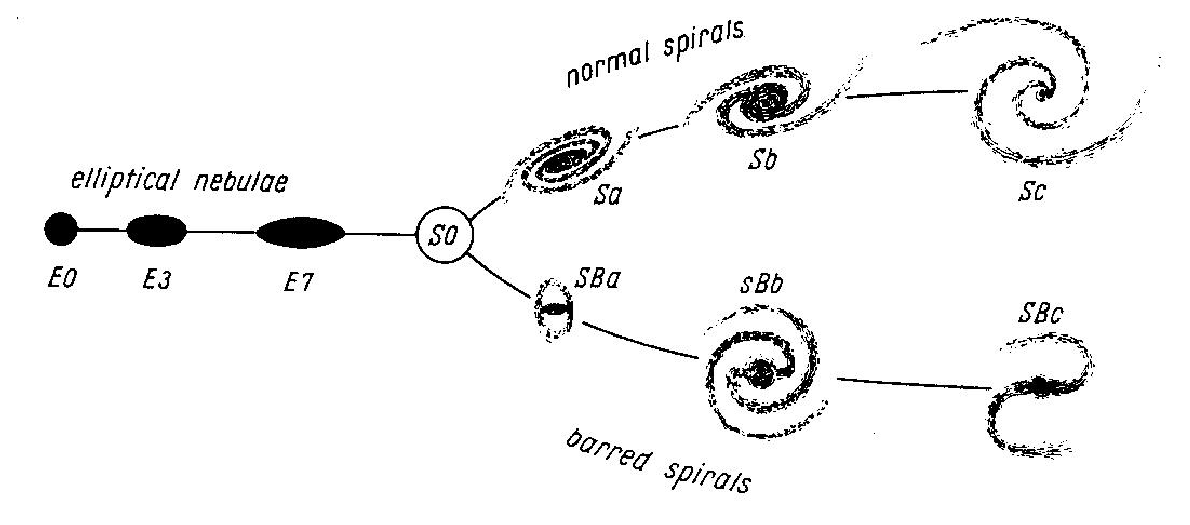
\includegraphics[width=5.5in]{tune.eps}


\cleardoublepage
\stepcounter{thelabs}
\noindent
{\hfill \Large {\bf Indoor Lab \#\labnum: Galaxy Classification} \hfill}

\noindent {\bf Objectives}:
\begin{itemize}
\item To understand the concept of \emph{color} in astronomy.
\item  To be able to classify galaxies based on their morphology and colors
\item  To investigate how galaxies evolve over time
\item  To search for, analyse and interpret information from large galaxy surveys including the Sloan Digital Sky Survey (SDSS)
\end{itemize}

\noindent
%{\bf Part 1. Virgo Cluster}
{\bf  Introduction}:

\begin{figure*}[ht]
        \begin{center}{\psfig{figure={Hubblefork.eps},width=10.0cm}}
        \caption{Hubble’s famous Tuning Fork diagram created by Dr Karen Masters, based on an activity designed by Las Cumbres Observatory Global Telescope Network (LCOGT).}\label{hubblefork}
        \end{center}
                \end{figure*}

\noindent

Edwin Hubble created the first classification of galaxies. He produced
a diagram, called the Tuning Fork diagram (Figure \ref{hubblefork})
based on features galaxies have in common. He came up with three
distinct groups - ellipticals, spirals and irregulars. Ellipticals
have no spiral arms or a disk and are classified by how round they
look, E0 is very round but an E7 is very flat. This number is actually
the ellipticity of the galaxy (the ratio of the semi major axis to the
semi minor axis). Spirals show a spiraling structure, spiral ``arms'',
and can be further split into barred (SB) and un-barred (S). They are
also classified by how tight their spiral arms are ``wound''. There is
a transition type called S0 which have no spiral arms but they have a
central bulge and a disk. Astronomers now use a slightly different
naming system with two major groups called early-type (including
ellipticals and S0s) and late-type galaxies (spirals).

Hubble thought that galaxies in time moved from left to right in his
Hubble Tuning Fork diagram over time, but we now know that this is
incorrect. Some galaxies move from right to left over time, and a much
smaller number from left to right sometimes, but there is no
inevitable progression of any individual galaxy across the diagram.

\noindent{\bf 2. The color of galaxies}

\noindent

The Sloan Digital Sky Survey SDSS has imaged a large portion of the
sky, and found more than 80 million galaxies. Classifying them by eye
would take huge amount of time. SDSS cleverly called upon the public
to help, and asked volunteers to look at images of new galaxies,
compare them with typical Early and Late type galaxies, and classify
the new objects accordingly. This project is called the \emph{Galaxy
Zoo}, {\tt http://www.galaxyzoo.org}. A quicker way to classify
galaxies, easier to implement in a computer, is by using their color.

\noindent {\bf Question:} Look at the Hubble Tuning Fork diagram reproduced above. How does the color differ for different galaxy types?



\begin{figure*}[ht]
        \centerline{\psfig{figure={SDSSgals.eps},width=18.0cm}}
        \caption{A selection of SDSS galaxies. }\label{SDSSgals}
         \end{figure*}


\noindent 
Figure \ref{SDSSgals} shows a selection of SDSS galaxies. The SDSS survey takes sky images in multiple filters. By combining these images color images of astronomical objects are obtained. 

\noindent First, look at each galaxy in Figure \ref{SDSSgals} and classify it according to its \emph{shape} according to both classification schemes: as \emph{early} or \emph{late} type, and as \emph{elliptical} E0-6, S0, \emph{spiral} S or SB a,b or c.

\vspace{20pt}

\noindent a \makebox[2cm]{\hrulefill}  \makebox[2cm]{\hrulefill}\makebox[1cm] d \makebox[2cm]{\hrulefill}  \makebox[2cm]{\hrulefill}\makebox[1cm] g \makebox[2cm]{\hrulefill}  \makebox[2cm]{\hrulefill}

\noindent b \makebox[2cm]{\hrulefill}  \makebox[2cm]{\hrulefill}\makebox[1cm] e \makebox[2cm]{\hrulefill}  \makebox[2cm]{\hrulefill}\makebox[1cm] h \makebox[2cm]{\hrulefill}  \makebox[2cm]{\hrulefill}

\noindent c \makebox[2cm]{\hrulefill} \makebox[2cm]{\hrulefill}\makebox[1cm] f \makebox[2cm]{\hrulefill}  \makebox[2cm]{\hrulefill}\makebox[1cm] i \makebox[2cm]{\hrulefill}  \makebox[2cm]{\hrulefill}

\vspace{20pt}


\noindent Now go to the SDSS Object Explorer Tool:

\noindent {\tt http://cas.sdss.org/public/en/tools/explore/obj.aspx}

\noindent and type in their coordinates (``Search by,'' at top
left). Click ``Save to Notes'' for each galaxy to save the information
automatically. Then you can just click on ``Show Notes'' to see your
measurements.  I mentioned that SDSS observed in \emph{multiple
filters} to obtain color information about astronomical objects. The
SDSS filters are: \u, \g, \r, \i \ and \z; \u \ is the bluest filter
and \z \ is the reddest.

\noindent 
You want to make a \emph{color-color diagram} of these galaxies. A
color-color diagram is a very useful astronomical tool: it is a plot
of one particular color, against another, for the same object.  In
astronomy colors are defined as difference in magnitude in different
filters. For this particular color-color diagram you want to plot the
SDSS \g-\r \ color, against the \u-\g \ color, i.e. \u-\g \ is on your
$x$-axis, \g-\r \ is on the $y$-axis. Now pay attention: because you
are using magnitudes, where the larger the number the brighter the
object, this may be counterintuitive:

\noindent {\bf Question:} Which is bluer: a galaxy with a larger value of \u-\g \ or with a lower value of \u-\g?

\noindent 
Use the box below for your color-color diagram. Mark the bottom-left
and top-right corner with the word BLUE or RED according to where you
expect the bluest and the reddest objects to fall. Draw an arrow that
indicates the direction in the plot in which objects get redder.

\noindent
Plot your \g-\r \ vs \u-\g \ colors in the box below. Briefly note
whether you see any patterns.


\begin{figure}[b!]
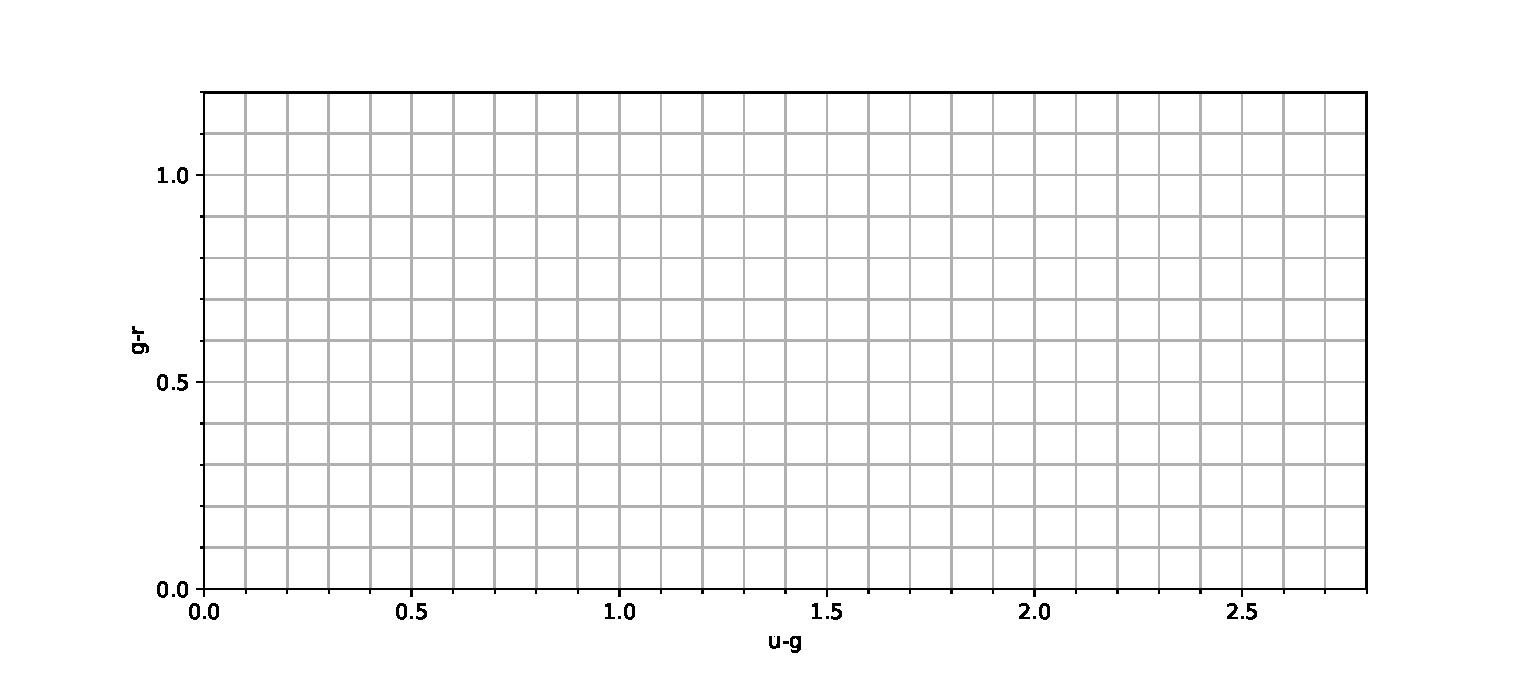
\includegraphics[width=0.99\textwidth]{colorcolor.eps}
\end{figure}

\clearpage

\noindent
Now draw a line $$y=-x+2.2.$$ This means draw a line the join points
that have $y$-axis value equal to 2.2 - the $x$-axis value. It was
found studying the SDSS sample that early type galaxies have ($u-r$)
values higher than 2.2, and late type galaxies have ($u-r$) values
lower than 2.2, indeed they are split by the equation ($g-r$) = $- (u-g)
+ 2.2$ (Strateva et al. 2001). Do you see this pattern in the data you analyzed? 

\bigskip
\noindent
Mark the box regions according to the type you expect them to host in the plot: mark the regions above and below your $y=x+2.2$ line with either EARLY or LATE, whichever you think is appropriate. 

%\begin{center}{\bf Extra credits/Homework}\end{center}

\noindent
{\bf 3. Clusters of galaxies}:

\noindent
George Abell classified \emph{thousands} of galaxy clusters, publishing them in 1958. We will use a few of them to see how galaxy colors change with redshift and draw conclusions about galaxy evolution!
The galaxy cluster Abell 2255 is at co-ordinates RA = 258.1292\deg\  and Dec = 64.092\deg .

\noindent
To obtain the colors of galaxies in Abell 2255, use the SDSS archive Navigation Tool: 

\noindent{\tt http://cas.sdss.org/public/en/tools/chart/navi.aspx}.

\noindent
You will need to type in the coordinates of the Abell 2255, click on ``Get Image'' and zoom out once or twice. Now click on roughly 20 galaxies that you think are part of the cluster (make a note of what criteria you use to decide if these are cluster members). On the right hand side of this webpage, you will see the colors listed for the galaxy you clicked on, write these down. You can click Save to Notes for each galaxy to do this automatically or do it by hand by typing/writing them. If you save the notes on the webpage just click on ‘Show Notes’ to see your measurements. You can export to CSV format if you wish to work on it in Excel, or any computational language, but that is not necessary.
Don’t forget, however, to include all of your measurements in your lab diary (stapled print-outs are fine).

\noindent
Important: think carefully about how you know which galaxies are part of Abell 2255, and which are just other galaxies at different distances in the same part of the sky. Briefly describe your 20 galaxies. Are they similar? How are they different? Make a color-color plot (as above) of your sample of Abell 2255 galaxies. Again, draw the line that ‘separates’ ellipticals from spirals. How many of these galaxies are ellipticals and how many spirals?



\clearpage

%\noindent
%{\bf Do Galaxy Colors Change with Redshift?}
%
%\noindent
%Now you have done this for a relatively nearby cluster (at a redshift of 0.081), try comparing the colors and classification of galaxies in clusters at different redshifts. The table below provides coordinates and redshift information fot three Abel clusters:
%
%\begin{table}[ht!]
%\begin{center}
%\begin{tabular}{l c c c}
%Name of cluster &  Redshift & RA (deg) & Dec (deg)\\\hline
%Abell 2255 & 0.081 & 258.129 & 64.093 \\ 
%Abell 0023 & 0.105 & 5.44 & -0.89 \\
%Abell 0267 & 0.230 & 28.77 & 1.01
%\end{tabular}
%\end{center}
%\caption{ Properties of the galaxy clusters used in this research project.}
%\end{table}
%
%\noindent
%Follow the same procedure as before to get the SDSS data on each cluster and create color-color plots. You will have to assume your sample contains no foreground or background galaxies. Count the \emph{fraction} of Early and Late type galaxies in each cluster. 
%\begin{itemize}
%\item{How does it change with the redshift? }
%\vspace{30pt}
%\item{What does that mean?}
%\vspace{30pt}
%\item{Can you comment in the light of this result on Hubble's initial prediction, that Galaxies would evolve rightward in his plot?}
%\vspace{30pt}
%\item{ Can you relate this result to what you know about \emph{stellar} evolution?}
%\end{itemize}



\cleardoublepage
\stepcounter{thelabs}
\noindent
{\hfill \Large {\bf Indoor Lab \#\labnum: The Deep Sky} \hfill}

\noindent Today we will use the Palomar Observatory Sky Survey
plates to investigate the deep sky.  You have used these before in the
Milky Way lab.  Here we will take a somewhat more careful look. 

Recall that the images are negatives so the light of the stars etc. is
dark. The images come in pairs, labeled ``E'' and ``O'' in the small
rectangle in the upper left. The images labeled E are taken with a red
filter -- so the image records the red light. The ones labeled O are
taken with a blue filter, and so records the blue light. With
each pair of images we will supply a transparent overlay.

Pick one of the available pairs supplied by your instructors.  {\bf
Please treat them with great care: keep them flat; no pencils or pens
or food near them, and do not write on paper on top of the
prints. Thanks!}

\noindent
{\bf 1. Orienting yourself in the image:} 

\noindent Each image is labeled in the upper left by an approximate
R.A.~and Dec of the center of the image.  Note that because of
precession the R.A. and Dec we would use is somewhat different than it
was in the 1950s when the images were taken. Nevertheless (most of)
the stars aren't moving fast in angle relative to each other, so we
can determine what the current R.A. and Dec is in this image.

\noindent First, write down the approximate center listed on your
image:

\vspace{40pt}

\noindent To do so, pick the four (roughly) brightest stars in the
image. Make sure the four are fairly widely separated on the page.
Using the given R.A. and Dec as a starting point, use Starry Night to
identify those four stars. List below their names, R.A.s, Decs and
magnitudes. Also, draw their rough configuration in the image on the
blank page at the end of the lab.

\noindent Remember: in the images, with the rectangle in the upper
left, North (higher Dec) is up and East (higher R.A.) is to the left.

\clearpage

\noindent {\bf 2. Using the coordinate grid}

\noindent With either the red or blue images, place the transparent
grid you received on top of the image. Align it such that the
North-South line goes through approximately the center, and that the
declinations of your identified stars are correct. Use the marking
tape to identify where each star is, so you can put the transparency
back into place quickly.

\noindent Using the R.A.s of the stars, determine the approximate
spacing of the thick and thin lines of right ascension. If there are
two thin-line spacings list both.

\vspace{100pt}

\noindent What is the center R.A. line of your grid?

\vspace{100pt}

\noindent In Starry Night, find a tenth magnitude star in the
field. Using your RA and Dec grid to help you, locate it in on the
POSS image. Mark your map at the end of the lab with its name and
location.  

\noindent In Starry Night, zoom in around that star to a 15 arcmin
field-of-view.  Make sure you have All Sky Image on and no magnitude
limits for the stars. Compare how many the stars you see in the POSS
image to those in Starry Night. Which shows more (and fainter) stars?

\clearpage

\noindent {\bf 3. Finding galaxies and nebulae}

\noindent These images have been chosen because they contain one (or
more) interesting objects that are either distant galaxies or clusters
in our own galaxy. Find one of these, determine its RA and Dec, and
draw it roughly below:

\vspace{100pt}

\noindent Is it red or blue? How does its form differ between the two
images? 

\vspace{80pt}

\noindent Using the RA/Dec grid, estimate its rough angular size:

\vspace{40pt}

\noindent Look it up in Starry Night by looking at that RA and
Dec. What is the name and classification of the object? What is its
physical size?



\cleardoublepage
\stepcounter{thelabs}
\noindent
{\hfill \Large {\bf Indoor Lab \#\labnum: Lenses and Telescopes} \hfill}

\noindent Today we will make a simple telescope using some lenses.  We
will begin by examining the properties of a lens, and learn how to
measure focal lengths. We will then use the lenses to make a
telescope, and examine its magnification.  

\noindent {\bf Equipment:} optical bench, magnetic stands, light
source, aperture mask, plane mirror, concave mirror, glass,
imaging screen, and several lenses. {\bf Make sure there is a plane
mirror.} 

\noindent
{\bf 1. Properties of a single lens} 

\noindent Set up the optical bench as follows, with the aperture mask
attached to the light source, a 70 mm lens and the screen, as shown
below. Position the source so the front face corresponds to the zero
position on the bench --- this makes measuring distances easier.

\begin{figure*}[h]
\centerline{\psfig{figure={uv.ps},width=13.0cm}}
\caption{}
\end{figure*}

\noindent In what follows, we shall refer to the distance between the
source and the lens as $v$ (the object distance), and the distance
between the lens and the screen (when the image is in focus on the
screen) as $u$ (the image distance). 

\noindent Move the lens so that $v= 60$ mm.  Then move the screen
until the image of the light source is in focus.  Determine the
corresponding value for $u$ and enter the result in the table below.
Repeat the procedure for the other values of $u$ given in the table.
Note as you proceed the relative brightness of the focused light at
each configuration --- mark whether the image is brightest for $v=20$
or $v=60$ mm.  Plot the results on the attached sheet of graph paper,
and join the points with a neat, smooth curve.
 
\begin{center}
\begin{tabular}{lc} \hline \\ [-6pt]
$v$ (mm)  & \hspace{1cm} $u$ (mm) \hspace{1cm} \\ [6pt]
\hline
60 &        \\ \hline
50 &        \\ \hline
40 &        \\ \hline
30 &        \\ \hline
20 &        \\ \hline
10 &        \\ \hline
\end{tabular}
\end{center}

\noindent On the schematic of the optics above, draw the path the
light takes from the center point of the aperture, assuming that the
light is in focus. Start at the arrows shown and continue the lines
until the light hits the screen. Remember the light goes straight when
going through the air and bends when it goes through the lens! Note of
course that not {\it all} of the light ends up going through the lens.

\noindent Mathematically, the relation between $u$, $v$ and the focal
length $f$ is given by the equation:

\begin{equation}
\frac{1}{u} + \frac{1}{v} = \frac{1}{f}
\end{equation}

\noindent A special case occurs when $u=v$.  Then:

\begin{equation}
\frac{1}{u}+\frac{1}{v} = \frac{1}{u}+\frac{1}{u} = \frac{2}{u}
=\frac{1}{f}
\end{equation}

\noindent In other words: $f=u/2$ when $u=v$.  From your plotted curve
find the point when $u=v$ and deduce $f$:

\vspace{30pt}

\noindent Examine your graph and comment:
\begin{enumerate}
\item What happens to $u$ as $v$ gets very large? \vspace{20pt}
\item What happens to $u$ as $v$ gets very close to $f$? \vspace{20pt}
\end{enumerate}
\noindent These special cases can be investigated with the above
equation.  When $v$ is very large (at infinity) then $1/v=0$.  What
then is the value of $u$?

\vspace{30pt}

\noindent When $v=f$ (i.e. the source is at the focus of the lens, what then is
the value of $u$?

\vspace{30pt}

\noindent {\bf 2. Parallel light and focal lengths}

\noindent We can use the results from part (1) in two ways: first, to
simulate on the optical bench a very distant light source, and then to
use this to directly measure focal lengths.

\noindent First, set up the optical bench as follows, with the light
source at one end as before, but now with the 48 mm focal length lens
and the plane mirror:

\begin{figure*}[h]
\centerline{\psfig{figure={parallel.ps},width=13.0cm}}
\caption{}
\end{figure*}

\noindent Adjust the position of the lens (keeping the mirror close to
it) so that the light from the source is reflected back off the mirror
and through the lens again, and is in sharp focus on the front face of
the source.  This may require some fiddling so you can actually see
the image on the source screen (if things are aligned too well, the
image will form on the aperture itself, where you won't be able to see
it).

\noindent Some thought should convince you that (a) the source-lens
distance is equal to the focal length of the lens, and (b) on removing
the mirror, the beam emerging from the lens will be equivalent to that
coming from a very distant object (that is, the rays will be
essentially parallel). 
Draw the light paths in the above diagram.

\clearpage

\noindent With a parallel (``collimated'') beam, we can directly
measure focal lengths of lenses.  Simply mount a lens on the bench in
the parallel beam close to the 48 mm lens, as follows:

\begin{figure*}[h]
\centerline{\psfig{figure={measure.ps},width=13.0cm}}
\caption{}
\end{figure*}


\noindent Adjust the position of the screen from the lens until a
sharp image is obtained.  From part (1) it should be clear hat this
distance equals the focal length of the lens. Compare your measurement
with the label on the lens itself:

\vspace{30pt}

\noindent Again, draw the light paths for an in-focus configuration in
the above diagram.

\noindent While we have a parallel beam set up, let us look at how a
mirror focuses a beam. Install the concave mirror and a piece of
straight, clear glass, as shown below:

\begin{figure*}[h]
\centerline{\psfig{figure={mirror.ps},width=13.0cm}}
\caption{}
\end{figure*}

\noindent Configure the mirror so that you can see the image form on
the {\it glass}. The distance between the concave mirror and the image
it forms from a parallel beam is its focal length.  Compare your
measured focal length to that stated on the mirror:

\vspace{30pt} 

\noindent Draw the paths of the rays in the figure above.

\noindent {\bf 3. A simple telescope}

\noindent Clear the optical bench of everything including the light
source, and mount two lenses: an ``objective'' lens O with focal
length $f_O$ and an ``eyepiece'' lens with focal length $f_e$. To
begin, put the eyepiece at one end, and position the objective length
a length $f_O$ from it. Try to look at a source on the far end of the
room; you will see that the telescope is not in focus.  Move the
objective back until the distant object is clearly in focus.

\begin{figure*}[h]
\centerline{\psfig{figure={telescope.ps},width=13.0cm}}
\caption{}
\end{figure*}

\noindent Draw the light paths in the diagram above.

\noindent If properly configured, this set up should produce a
magnified image of distant objects --- if you find that the images are
{\it demagnified} how do you have to change the configuration? 

\vspace{30pt}

\noindent Measure the distance from lens O to lens E.  How does that
compare with the number you expect? 

\vspace{30pt}

\noindent We now have a telescope that magnifies distant objects.
According to the theory, the angular magnification of the telescope is
given by $M=f_O/f_e$.  Using the labeled values of $f_O$ and $f_e$ on
your lenses, calculate the theoretical magnification of the telescope.

\vspace{30pt}

\noindent Now pick a different lens for the objective, and report if
the magnification changes in the expected manner:

\vspace{50pt}


\noindent {\bf 4. Extra credit}

\noindent Notice that the image in the telescope we have built is
reversed.  Suggest and implement a change in the design to make the
images upright.

\clearpage



\cleardoublepage
\stepcounter{thelabs}
\noindent
{\hfill \Large {\bf Indoor Lab \#\labnum: Stellar Spectra} \hfill}

\noindent Today we will examine the colors, the ``spectra,'' and the
velocities of stars. Most of the stars we will look at are {\it much}
fainter than you can see with your eye --- however, they are very
similar physically to those you are familiar with, just further away
in our Galaxy. We will also take a look at a handful of galaxies, and
try to understand how the stellar content of the galaxies affects
their images and spectra.

\noindent Below is a spectrum of the Sun, in black, and a blackbody
spectrum at T=5777 Kelvin in green. Notice how the peaks coincide:
this indicates that the temperature of the sun is close to a
temperature of T=5777 Kelvin, and notice the features in the sun
spectrum: absorption and emission from various elements, while the
blackbody spectrum is smooth.

\begin{figure*}[h!]
\begin{center}{\psfig{figure={Sunspec.eps},width=10.0cm}} \caption{A
spectrum of the Sun.}
\end{center}
\end{figure*}

\noindent To begin, open a Mozilla Firefox browser on your computer to
the URL {\tt http://data.sdss.org}.  This site gives you access to a
set of real astronomical data publicly released by a team of
astronomers (including us at NYU).  In the menu, go to ``Optical
Spectra'' and under that ``Bulk Search.''

\noindent
{\bf 1. Colors of stars}

\noindent Enter the right ascensions and declinations listed below
into the ``bulk search'' form. Use a ``Search Range'' of 0.05
arcminutes. When you submit the search, it should return a table of
rows.  Each row corresponds to a star, and by hitting ``Plot'' in the
appropriate row you can look at the image and the spectrum of the
star. You can also hit ``CAS'' which will open a new tab, that also
shows the image of the object.

\begin{center}
\begin{tabular}{ccccccc} \hline \\ [-6pt]
R.A. (deg)  & Dec (deg)  & \hspace{0.2cm} Type \hspace{0.2cm} 
& \hspace{0.2cm} $\lambda_{\mathrm{peak}}$ (Ang.) \hspace{0.2cm} 
& \hspace{0.2cm} T (K) \hspace{0.2cm} 
& \hspace{0.2cm} H\&K? \hspace{0.2cm} 
& \hspace{0.2cm} Balmer?  \hspace{0.2cm} 
\\ [6pt]
\hline
228.06551 &  6.865659 & & & & &    \\ \hline
16.437201 &  -10.7071  & & & & &   \\ \hline
17.848558 &  16.327376 & & & & &    \\ \hline
151.95765 &  34.369592 & & & & &    \\ \hline
47.249486 &  38.01783  & & & & &   \\ \hline
64.948151 &  5.261293  & & & & &   \\ \hline
146.77222 &  62.631055 & & & & &    \\ \hline
\end{tabular}
\end{center}

\noindent First consider just the colors of the stars in the image on
the bottom left.  

\noindent Note that these images, in addition to
being far deeper than what you can see with your eye, exhibit somewhat
more color contrast as well.

\noindent Under the ``Type'' column, rank the list above from bluest
to reddest according to the image that you see. Use the labels O, B,
A, F, G, K, M from bluest to reddest.

\noindent The bluer of the stars are the hotter ones, and usually the
more massive and younger stars as well.  

\noindent
{\bf 2. Relationship of colors to the spectrum}

\noindent Now consider the ``spectrum'' shown on each plot.  The
curve shown is the amount of light emitted from each wavelength, from
blue (short) wavelengths on the left to red (long) wavelengths on the
right.  The unit of length here is the Angstrom, which is $10^{-10}$
meters. Your eye is sensitive to light between about 4000 and 7000
Angstroms.

\noindent For a perfect ``blackbody'' spectrum, the temperature of a
star would be related to its peak wavelength of emission by the simple
formula: $\lambda_{\mathrm{peak}} T \approx 3$ mm Kelvin. Although
stars are not perfect blackbodies, there is still an approximate
relationship between the color and the temperature.

\noindent Look at each spectrum and estimate the peak wavelength.  If
the spectrum continues to increase past the left or right edge of the
spectrum, indicate the maximum or minimum possible wavelength. 

\noindent Use the peak wavelength to deduce the temperature (or the
minimum or maximum temperature where appropriate).  Notice that the
temperature is closely related to the color classification in the
first section. This temperature is the effective temperature at the
surface of the star --- for all these stars the temperatures in their
centers where nuclear fusion is occurring is much hotter!

\noindent
{\bf 3. Features in the spectra}

\noindent There are a number of clear absorption features (called
``lines) in the spectra, seen as deep troughs at particular
wavelengths. There are many sets of lines associated with a number of
different absorption features, but we'll be interested today in just
two sets of them: the calcium H and K lines, and the hydrogen Balmer
lines.

\noindent The calcium H and K lines are near the left edge of these
spectra, at around 3933 Angstroms (K) and 3969 (H) Angstroms. They are
produced by trace amounts of calcium (gaseous calcium!) in the outer
atmospheres of the stars. Look for these in the spectra and mark the
table above according to whether each star has visible H \& K.  Which
star has the strongest calcium features?

\noindent The Balmer lines are features due to hydrogen in the outer
atmosphere. There is a large set of them: H$\alpha$ at 6563 Angstroms,
H$\beta$ at 4861 Angstroms, H$\gamma$ at 4341 Angstroms, H$\delta$ at
4102 Angstroms, H$\epsilon$ at 3970 Angstroms, etc.  Note in the above
table which stars have these, and which star has the strongest
features.

\noindent 
There is always hydrogen in stellar atmospheres, but it has to be at
the right temperature to produce deep hydrogen lines. Using the table
above, guess what that temperature is.

\vspace{30pt}

\noindent Which type(s) of stars have neither H \& K lines nor Balmer
lines?

\vspace{30pt}

\noindent
{\bf 4. Doppler shifts in galaxies}

\noindent Now we will look at a handful of galaxies.  As you probably
know, galaxies are distant analogs to the Milky Way, and consist of
conglomerations of 10s of billions of stars. This fact will be evident
when we look at their spectra. Search for the following spectra in the
``bulk search'' window (but keep your results window for the stars
open for comparison). 

\begin{center}
\begin{tabular}{ccccccc} \hline \\ [-6pt]
R.A. (deg)  & Dec (deg)  & \hspace{0.02cm} Star type \hspace{0.02cm} 
& Young/old?
& \hspace{0.02cm} K line (Ang.) \hspace{0.02cm} 
& \hspace{0.02cm} H$\delta$ (Ang.) \hspace{0.02cm} 
& \hspace{0.02cm} Velocity (km/s) \hspace{0.02cm} 
\\ [6pt]
\hline
153.4605 &  38.764896 & & & \\ \hline
140.03594 &  8.1503628 & & & \\ \hline
35.170815 &  1.0521941 & & & \\ \hline
185.7200 &  6.6798709 & & & \\ \hline
173.41101 &  4.1961732 & & & \\ \hline
\end{tabular}
\end{center}

\noindent You will notice for some galaxy there are large ``spikes,''
which we call ``emission lines.'' The light at these wavelengths is
not coming from the stars, but instead from gas in HII regions within
the galaxy --- their presence is usually a sign of ongoing
star-formation in the galaxy (though certain lines indicate the
presence of a black hole at the center of the galaxy).  Note that the
most prominent set of lines are Balmer {\it emission} lines!

\noindent Look for the H and K lines of calcium and the Balmer lines
for each spectrum.  Because Balmer emission makes it hard to see the
lines, you will have to search for Balmer emission in the H$\delta$
line to see it in the cases where it is there.  List above the
location in the spectrum of the K line and the H$\delta$ line in cases
where you see them. 


\begin{figure*}[h]
\centerline{\psfig{figure={doppler.eps},width=13.0cm}}
 \end{figure*}

\noindent These galaxies are moving quickly away from us. Remember 
that light travels at a finite speed.  Just like the sound of a siren
is affected by the relative motion of the siren (the source) and us
(the listener), the motion of celestial objects away from us modifies
the frequency of the light emission. When an ambulance drives toward
us the sound will be higher pitched: higher frequencies and lower
wavelengths. When the ambulance moves away the frequency decreases and
the wavelength gets larger. This is a purely geometric effect: look at
the figure in the next page to visualize it. Similarly, these galaxies
are receding from us due to the expansion of the universe, and the
light they emit will appear at a larger wavelenth than it was emitted
at: it will be ``reddened''. We call this ``cosmological redshift''.
Therefore, you will notice that the wavelengths of these lines are
{\it redshifted} from their positions in the stellar spectra, which
are almost at rest with respect to us. This Doppler shift is related
to the velocity by the equation:

\begin{equation}
\frac{\lambda_{\mathrm{obs}}}
{\lambda_{\mathrm{rest}}} = 1 + \frac{v}{c}
\end{equation}

\noindent where $c=299792$ km/s is the speed of light. Use this
equation to deduce the velocities of recession for the galaxies above,
and list it in the table.

\noindent
{\bf 5. Colors of galaxies}

\noindent Compare the spectra of the galaxies to the spectra of the
stars.  Write down which type of star each galaxies spectrum is most
similar to. The bluest stars are the shortest-lived, and the reddest
stars are the longest lived --- based on this fact write down whether
each galaxy is young or old (consider O, B and A stars ``young'' and
any cooler star to be ``old''). To put these ``ages'' in perspective,
A stars live for a billion years!

\noindent Look at the colors in the images of the galaxies --- you
should be able to notice that the ``younger'' galaxies are in general
bluer than the ``older'' galaxies.

\noindent Look up the galaxy at RA $=$ 215.08136 and Dec $=$
3.9327125. Click on the image on the bottom left to get a larger
view.  In general, where does the star-formation in the three big
galaxies you see seem to be occuring? Nearer their centers or further
out?

\vspace{30pt}

\noindent
{\bf 6. How faint are these stars and galaxies?}

\noindent The images and spectra you looked at in this lab are MUCH
fainter than visible with the human eye --- they were obtained with a
2.5-meter telescope. To get a sense, enter the coordinates of the star
Castor (RA $=$ 113.65, Dec $=$ 31.888) into the Navigate page for CAS
({\tt http://skyserver.sdss.org/dr15/en/tools/chart/navi.aspx}); this
is the same imaging you were looking at for the earlier objects in
this lab. Castor is about as bright as Polaris.  You will need to zoom
back in the image to see what is going on. Castor is much brighter
than all of the other objects we have been looking at!

\clearpage



\cleardoublepage
\stepcounter{thelabs}
\noindent
{\hfill \Large {\bf Outdoor Lab \#\labnum: A First Look at the Stars} \hfill}

\marginpar{
\vspace{-1.6cm}
\hfill 00$\deg$\makebox[2cm]{\hrulefill} \\
\vspace{-0.028cm}
\hfill 01$\deg$\makebox[2cm]{\hrulefill} \\
\vspace{-0.028cm}
\hfill 02$\deg$\makebox[2cm]{\hrulefill} \\
\vspace{-0.028cm}
\hfill 03$\deg$\makebox[2cm]{\hrulefill} \\
\vspace{-0.028cm}
\hfill 04$\deg$\makebox[2cm]{\hrulefill} \\
\vspace{-0.028cm}
\hfill 05$\deg$\makebox[2cm]{\hrulefill} \\
\vspace{-0.028cm}
\hfill 06$\deg$\makebox[2cm]{\hrulefill} \\
\vspace{-0.028cm}
\hfill 07$\deg$\makebox[2cm]{\hrulefill} \\
\vspace{-0.028cm}
\hfill 08$\deg$\makebox[2cm]{\hrulefill} \\
\vspace{-0.028cm}
\hfill 09$\deg$\makebox[2cm]{\hrulefill} \\
\vspace{-0.028cm}
\hfill 10$\deg$\makebox[2cm]{\hrulefill} \\
\vspace{-0.028cm}
\hfill 11$\deg$\makebox[2cm]{\hrulefill} \\
\vspace{-0.028cm}
\hfill 12$\deg$\makebox[2cm]{\hrulefill} \\
\vspace{-0.028cm}
\hfill 13$\deg$\makebox[2cm]{\hrulefill} \\
\vspace{-0.028cm}
\hfill 14$\deg$\makebox[2cm]{\hrulefill} \\
\vspace{-0.028cm}
\hfill 15$\deg$\makebox[2cm]{\hrulefill} \\
\vspace{-0.028cm}
\hfill 16$\deg$\makebox[2cm]{\hrulefill} \\
\vspace{-0.028cm}
\hfill 17$\deg$\makebox[2cm]{\hrulefill} \\
\vspace{-0.028cm}
\hfill 18$\deg$\makebox[2cm]{\hrulefill} \\
\vspace{-0.028cm}
\hfill 19$\deg$\makebox[2cm]{\hrulefill} \\
\vspace{-0.028cm}
\hfill 20$\deg$\makebox[2cm]{\hrulefill} \\
\vspace{-0.028cm}
\hfill 21$\deg$\makebox[2cm]{\hrulefill} \\
\vspace{-0.028cm}
\hfill 22$\deg$\makebox[2cm]{\hrulefill} \\
\vspace{-0.028cm}
\hfill 23$\deg$\makebox[2cm]{\hrulefill} \\
\vspace{-0.028cm}
\hfill 24$\deg$\makebox[2cm]{\hrulefill} \\
\vspace{-0.028cm}
\hfill 25$\deg$\makebox[2cm]{\hrulefill} \\
}


\bigskip

\noindent
{Objective:} To find our way around the sky by identifying the
brightest stars and constellations, and by measuring some angles
in the sky.

\bigskip\noindent
{\bf INSIDE PREPARATIONS}
\bigskip

\noindent
{\bf 1. Review of tonight's sky}

\medskip
\noindent
Outside we are going to first use a simple map of the sky, shown in
Fig.~1.  The map is to be held above your head and tilted down to the
horizon in the direction you are looking. The map is suitable for use
around September at about 8pm standard time.

Identify a few of the main constellations in the map using the M5
atlas (e.g., Cygnus). If there are any bright planets visible,
the instructor will give you their coordinates: using the M5 as a
guide to the RA and Dec lines, draw them in on Fig.~1.

Examine map 1 in the M5 atlas, centered on Polaris which lies within
1\deg\ of the North celestial pole (NCP). Note the position of Polaris
with respect to the W of Cassiopeia and the pointers Merak and Duhbe
of the Big Dipper in Ursa Major. Note also the hour markers around the
outside of the map.

\bigskip
\noindent
{\bf 2. Measuring angles}

\medskip
\noindent
An important aspect of locating and
identifying celestial objects is their positions. There is no
perception of depth in space, but we can describe the apparent
position of a star or planet using angles. For example, we can specify
the angle between two stars, or the altitude (Alt) and azimuth (Az) of
a single star. Recall that Alt is the angle from the horizon up to the
star, and Az is the angle from the North horizon (measured Eastwards)
to the point on the horizon immediately beneath the star. In all these
cases, the ``angle'' means the angle between lines in the two
directions that meet at us, or at our eyes.

One rough way to measure large angles is to point with straight arms
in the two directions at the same time, and to estimate the angle
between your arms.

A second way is to remember some typical angle sizes: e.g.,  at
arms length, the width of a fist including your thumb is about 10\deg\
and the width of your little finger is about 1\deg.

A more accurate way to measure angles is with some kind of measuring
device. We shall use a simple angle ruler that, when held at arm's
length at right angles to your arm, will measure angles.

Simple trigonometry tells us that the angle $\theta$ (in degrees)
subtended at our eye by an object of size $s$ (across our line of
sight) at a distance D from us, is given by the formula $\theta =
(360/2\pi)\,s/D$ or $57.3\, s/D$, when the angle is not too large.
For $\theta$ equal to 1\deg, then $D = 57.3\, s$.  We use this to
construct an angle ruler.  It turns out that the distance from my eye
to my outstretched hand is about 57~cm, and this is a reasonable approximation
for most ordinary sized people. Thus from the formula, a length ($s$) of
1~cm held across the line of sight is not a bad approximation to an
angle of $1\deg$.  Down the side margin of the front page I have
marked intervals of 1~cm and labeled them in degrees.

Now you can use this ruler to measure the angle between two points or
stars. Hold it at arm's length, at right angles to your line of
sight. Line the zero position up with one star, and read off the angle
where it matches the other star.

Use your angle ruler to check the finger and fist estimates given
above. Unless you have unusual hands or arms, the angles should be
fairly close to those given.

\medskip
\bigskip\noindent
{\bf AT THE OBSERVATORY}
\bigskip


\noindent 
Take a look around the sky and identify some of the brightest stars
and constellations. Circle the constellations you recognize in
Fig.~1. 
Locate your zenith (Alt = 90\deg) and convince yourself that you
could see half the celestial sphere down to the horizon, if it wasn't
for the city buildings.

\bigskip\noindent
{\bf 3. Polaris}

\bigskip\noindent
Using the star maps locate Polaris. It is not so easy to find as it is
fairly faint and the city lights of mid town are bright. It lies
30\deg\ from the W of Cassiopeia and the pointers of the Big Dipper.

Once you can see Polaris you know (roughly) where the NCP is, and the
direction of due North on Earth (the horizon point directly below
Polaris). Keep walking in this direction and you will eventually reach
the North pole. You will notice that contrary to common belief, the
avenues of Manhattan (and Broadway in our part of town) are not
oriented N--S.
          
\noindent Measure as accurately as possible the altitude of Polaris. You cannot
see the exact horizon so start from one arm held accurately
horizontal. Your angle ruler will not be long enough so you will need
to place more than one, end to end to build up the height.

\bigskip
{\hfill Alt of Polaris = \makebox[4cm]{\hrulefill} \hfill}

\clearpage

\noindent Use your binoculars, and look at Polaris through them. Can you verify
you are actually looking at Polaris?  It takes some practice to know
how bright a star should look through the binoculars. Draw the field
of stars centered on Polaris as you see it in the binoculars:

\centerline{\psfig{figure={o4s_f2.eps},width=4.5cm}}


\bigskip\noindent
{\bf 4. Altitude and Azimuth}

\bigskip\noindent
Locate and measure the Alt and Az of the objects in the following
table. For Alt use the angle ruler, for Az use the arm
method. Remember Az is measured from North (below Polaris) through East.

\noindent Vega's azimuth will be a bit tricky to estimate since it is near
zenith. As it transits its azimuth changes quickly by almost 180
degrees over a short period of time.

\begin{center}
\begin{tabular}{lcc} \hline \\ [-6pt]
Star   &\hspace{1.5cm} Altitude \hspace{1.5cm} & \ \ Azimuth \ \ \ \
 \\ [6pt]  \hline
Vega    &   &        \\ \hline
Deneb    &   &       \\ \hline
Altair    &   &       \\ \hline
\end{tabular}
\end{center}

\bigskip\noindent
{\bf 5. Angular separation}

\bigskip\noindent
Locate and measure with your ruler the angular separation of the following.
Note too, which is the brighter of each pair. If you cannot find one
of the pairs, just write that down. 

\begin{center}
\begin{tabular}{lccc} \hline \\ [-6pt]
Pair   & \hspace{1cm} Separation \hspace{1cm}& Brighter Component \\ [6pt]
\hline
Deneb -- Vega      & &        \\ \hline
Sadr -- Deneb     & &       \\ \hline
Hercules's shoulders       & &       \\ \hline
\end{tabular}
\end{center}

\noindent Using these estimates, estimate the field-of-view of the binoculars
you are using.

\clearpage 
\medskip\noindent
{\bf 6. Colors}

\bigskip\noindent 
The colors of stars are subtly different. 
They are typically described as: blue-white, white,
yellow-white, yellow, orange, red.  Describe the colors of the following.
  
\begin{center}
\begin{tabular}{lcc} \hline \\  [-6pt]
Star   &\hspace{1.5cm}  Color \hspace{1.5cm} &  \\  [6pt]
\hline
Deneb    &   &        \\ \hline
Vega     &   &       \\ \hline
Sadr     &   &       \\ \hline
Altair    &   &       \\  \hline
Caph    &   &       \\  \hline
\end{tabular}
\end{center}


\medskip\noindent
{\bf 7. Star time}

\bigskip\noindent
Study the sky near Polaris using the M5 map~1.  
The circles are lines of Declination and 
and the radial lines are lines of Right Ascension, marked around the 
outside in hours. Compare the map with the sky and
orient it so that they match up. Read the RA grid marker that is
highest in the sky. 

\medskip
{\hfill RA = \makebox[4cm]{\hrulefill} \hfill }

\medskip
This line of RA runs from Polaris through the zenith to the South
horizon. Its value is called the sidereal time. As the sky turns its
value increases like a clock. 

\bigskip\noindent
{\bf 8. Magnitudes}

\bigskip\noindent Compare Cygnus
with the detailed star maps in the M5 atlas.

Find the faintest star you can just see in the sky in this region. Read its
magnitude from the atlas:  \makebox[4cm]{\hrulefill}

\smallskip\noindent
Find a faint star in the atlas in this region that you cannot see with
your naked eye.
 
What magnitude is it: \makebox[4cm]{\hrulefill}
 
Locate it with binoculars. Can you see it now: \makebox[4cm]{\hrulefill}


\newpage

\begin{figure*}[h]
        \centerline{\psfig{figure={September.001.eps},width=8.5in,angle=90.}}
        \caption{}
         \end{figure*}


\cleardoublepage
\stepcounter{thelabs}
\noindent
{\hfill \Large {\bf Outdoor Lab \#\labnum: Dialing in the Stars} \hfill}

\noindent
{Objectives:} To introduce some practical aspects of using an
astronomical telescope. If the weather is clear, we will aim to do
this whole lab. If the weather is cloudy (but without precipitation)
we will perform the telescope setup aspects of the lab but not look at
stars.

\bigskip\noindent
{\bf INSIDE PREPARATIONS\\
(DO NOT HAND THIS SECTION IN---KEEP FOR FUTURE REFERENCE!}

\medskip
\bigskip
\noindent
{\bf 1. Telescope basics}

\medskip
\noindent
\emph{Optics}. The telescopes we will use today are ``equatorial''
telescopes, and have an aperture of 10 inches diameter, which allows
them to collect much more light than the human eye (about 1000 times
more) so that we can see much fainter objects.  The optics are quite
complicated. At the front is a transparent plate, and in the center a
small secondary mirror pointing inwards. The main optical component is
a converging mirror at the other end of the telescope. The light from
a distant star passes through the glass plate, bounces off the primary
mirror, comes back up the tube, is reflected back down the tube by the
secondary and passes through a hole in the primary mirror to the
eyepiece.

\medskip \noindent
\emph{Focus}.
There is a knob on the back of the telescope that focuses the optics
(this is the longer knob; the shorter one locks and unlocks the
primary mirror and should not be touched). Once set up, the focus knob
does not need to be adjusted unless you change the eyepiece.

\medskip \noindent
\emph{Magnification}. When you look through the eyepiece the
view is magnified. We will not be concerned with this aspect today,
but for completeness note that the magnification is given by
the formula $m = f_o/f_e$ where $f_e$ is the focal length of the
eyepiece and $f_o$ is the focal length of the objective or primary
optical component. $f_e$ is usually written on the eyepieces in
mm. $f_o$ for our telescopes is about 2500 mm. So for a 25 mm
eyepiece the magnification is 2500/25 = 100.

\medskip \noindent 
\emph{Finder}. Attached to the side of the telescope is a
small finder telescope---it acts a bit like the sights on a rifle. It
has a magnification of 6, and sees about 5\deg\ of the sky---much more
than through the main eyepiece. When you look though the finder there
is a cross hair, that should be aligned so that a star on the cross
hair appears in the eyepiece. Thus one way to observe a star is to
line up the telescope roughly in the direction of the star; then line
up the star in the finder. It should then appear in the main
eyepiece. If it does not, the finder requires adjustment with the
small screws holding it in place, which you should ask the instructor
to perform.

\medskip \noindent 
\emph{Control}. The telescopes we will use have two moving axes that
correspond to the sky coordinates RA and Dec. Each axis has a scale
which enables you to dial in and point at a star of known
coordinates. The Dec circle appears just on one side of the telescope
and is marked in degrees; the opposite circle is unmarked. The RA
circle is marked in hours, with smaller 5 min ticks.

\medskip\noindent Each axis has a brake. The Dec brake is on the
unlabeled circle; the dial in the center of the circle screws and
unscrews. The RA brake is the silver lever next to the RA adjustment
knob.

\medskip\noindent To move over large angles: release the axis brake;
move the telescope; then reset the break gently---not tightly. For
precision setting, there are control knobs for each axis that move the
telescope over small angles.

\noindent
A correctly set up telescope can move in RA and Dec because it is
mounted at an angle so that one axis is aligned with the polar
axis. When you turn the telescope about this axis you are turning it
in RA; when you turn it about the other axis you are turning to
different Decs at the same RA. When you have set on a star, a motor
inside the telescope turns the polar axis to keep track of the star
(i.e., it keeps it pointing to the same RA and so compensates for
Earth's rotation).

\noindent
We also have on the roof several 10 inch diameter telescopes of the
``alt-az'' variety (rather than equatorial).  These telescopes do not
track without using their electronic devices (which we won't
do). However, they are fun to use and we may use them in later labs.

\medskip\noindent
Before going out, review the recipe below as you will have to do it
outside. Also please remember:

\bigskip
\centerline{\bf Don't touch any part of the telescope optics} 

\medskip
\centerline{\bf Don't force any mechanical part of telescope} 

\medskip
\centerline{\bf Only put the axis brakes on gently}

\medskip
\medskip
\bigskip
\noindent
{\bf 2. Recipe for setting up telescope}

\medskip\noindent (a). First choose an eyepiece.  Recall that you will
want to be able to easily find your bearing, so you do not want a very
high magnification image---thus you want a long focal length
eyepiece. The instructors will give you a tour of the lab room when
you arrive on the roof, and tell you where everything is.

\medskip\noindent (b). Turn on the telescope with the small switch on
the left, making sure the electronic paddle is attached. If it does
not turn on, it is out of battery and/or needs to be plugged in; ask
the instructor for help. Once on, wait for the telescope to finish its
initialization sequence. It will say something like ``0 to align, MODE
for settings.'' DO NOT PRESS ``0.''

\medskip\noindent (c). Using the paddle, press MODE. Use the up and
down arrow keys near the {\it bottom} of the paddle (not the ones near
the top) and the ENTER key to navigate to SETUP. If you press ENTER
and use the arrows, you should be able to find the following settings:
\begin{itemize}
\item DATE (set it to the date)
\item TIME (set it to the current STANDARD time)
\item DAYLIGHT SAVING (set it to NO)
\item TELESCOPE, under which are:
\begin{itemize}
  \item MOUNT (set it to POLAR)
  \item TRACKING RATE (set it to SIDEREAL)
  \item GPS ALIGNMENT (set it to OFF)
\end{itemize}
\item SITE (set it to NEW YORK)
\end{itemize}
Very likely the telescope will already have these settings, but you
should double check!

\medskip\noindent
(d). Locate Polaris with the naked eye. (If it is cloudy, we are just
going to pretend we know where it is).

\medskip\noindent
(e). Rotate the telescope about the Dec axis so that it reads
90\deg.

\medskip\noindent (f). Turn the whole tripod of the telescope until
the leg parallel to the RA axis points at Polaris. (If it is cloudy,
we are just going to pretend it is pointing correctly already).

\medskip\noindent
(g). Make sure the wedge angle of the mount below the telescope is at
41 deg. If it is not, ask the instructor for help fixing it.

\medskip\noindent (h). Level the telescope by adjusting the legs and
using the spirit (or ``bubble'') level on the tripod. 

\medskip\noindent (i).  Find Polaris in the finder, If it is off to
one side or not visible, readjust the tripod so that Polaris falls
close to the cross hair in the finder. At this stage you do not have
to be too precise; just make sure that Polaris roughly in middle of
the finder. (If it is cloudy, skip this step).

\medskip\noindent (j). Using the paddle, navigate to ALIGN, and follow
these steps:
\begin{itemize}
\item It should show EASY; using the arrows, change it to ONE STAR and
press ENTER. It should now display POLAR ALIGN; some instructions
appear (which you don't have to wait for).
\item Move the HA indicator on the RA circle to its zero position at
the bottom of the telescope. 
\item Press ENTER. The telescope will move, as it tries to center on
Polaris (which is slighly off the pole).
\item Now readjust the tripod with precision, by turning the tripod,
and releveling it, to center Polaris in the finder and the eyepiece to
the best of your ability. If Polaris remains always much too high or
too low in the finder, consult the instructor. DO NOT MOVE THE DIALS
OF THE TELESCOPE AXES! (If it is cloudy, skip this step).
\item Press ENTER. The telescope will move towards a bright star that it
chooses based on the time of night and the date to be in the sky
(e.g. Vega or Betelgeuse).
\item When it is done slewing, adjust the RA and Dec dials to center the
star. Press ENTER. (If it is cloudy, skip this step).
\end{itemize}

At this point, the telescope will be calibrated and will start to
track at the sidereal rate. DO NOT MOVE THE TRIPOD AT ALL AFTER THIS
POINT: you now will point at different stars just by adjusting the RA
and Dec axes of the telescope.

\medskip\noindent
(k) With the star centered, slide the RA circle with the hours labeled
around until the RA reads the RA of the star. There are two sets of
numbers increasing in opposite directions---one for the Northern
Hemisphere and one for the Southern Hemisphere---think about their
direction and use the right set! The Dec should already be OK to
within a degree or so.

\medskip\noindent
It is done: the setting circles roughly correspond to RA and
Dec on the celestial sphere. A star of known coordinates can be found
by moving the telescope until the dials read correctly (this should
be accurate enough to place the star in the finder). Conversely, the
coordinates of a star can be found by centering it, then reading the
dials. Remember---be gentle with the brakes.


\clearpage
\noindent
{\bf OUTSIDE (TO HAND IN)}

\bigskip\noindent
{\bf 3. Measuring Coordinates}

\medskip\noindent
Measure the coordinates of each of the stars in the table below. In
turn: locate the star by eye (e.g., using the sky maps in the Mag 5
atlas); move the telescope so that the star is centered first in the
finder, then in the eyepiece; read off the star's coordinates from the
setting circles to within 5 min and 1\deg\ in RA and Dec,
respectively.

\begin{center}
\begin{tabular}{lcc} \hline \\ [-6pt]
\hspace{1cm}Name\hspace{1cm} &  \hspace{1cm} Your measured:  RA \hspace{1cm} & Dec \\ [6pt]
\hline
a) Altair  & &     \\ \hline
b) Vega  & &  \\ \hline
c) Deneb  & &    \\ \hline
d) Caph  & &   \\ \hline
  \end{tabular}
\end{center}

\bigskip\noindent
{\bf 4. Dialing objects}

\bigskip\noindent The table below lists the coordinates of four
objects. Dial them in on the setting circles and report what you see
at these locations. If you don't see anything obvious on the first
one, you probably have set up your telescope wrong!

\begin{center}
\begin{tabular}{lcc} \hline \\ [-6pt]
 \hspace{1.5cm}  RA \hspace{1cm} & Dec \hspace{1cm}& \hspace{3cm}Report\hspace{3cm} \\ [6pt]
\hline
a) 21h~44m  & $+9^\circ$ 52$'$ &     \\ \hline % Enif (mag 3 star)
b) 22h~22m  & $+57^\circ$ 7$'$ &     \\ \hline % Double Cluster
c) 21h~39m  & $+57^\circ$ 30$'$ &  \\ \hline % Elephant's Trunk
d) 0h~43m   & $+41^\circ$ 16$'$ &    \\ \hline % Andromeda
  \end{tabular}
\end{center}


\cleardoublepage
\stepcounter{thelabs}
\noindent
{\hfill \Large {\bf Outdoor Lab \#\labnum: First observations} \hfill}

\noindent
{\bf 1. Finding Objects.}  

\noindent The best technique for finding an object depends on how
bright it is. In this lab we will begin with objects which are naked
eye, or small offsets from bright stars. We will use the equatorial
telescopes. In subsequent labs we will try more difficult cases.

\medskip\noindent In particular, for this lab, we will only rely on
the Edmund atlas.  As you will see later, this is insufficient for
finding anything not very close to a reasonably bright star.

\medskip\noindent As you proceed below, for each object begin with a
long eyepiece, so a large field of view, when you are first trying to
find it. Once you have centered the object of interest using that
eyepiece, you can insert a smaller one for a more magnified view if
desired.

\medskip\noindent Note that the image is \emph{inverted} -- upside
down -- in the finder, but \emph{upright} in the main eyepiece. It is
also important to have a good idea of the size of the patch of sky
you are looking at. In the finder, this is about 7\deg, and in the
main eyepiece it is much smaller.

\bigskip
\bigskip
\bigskip
\noindent
{\bf 2. Magnification and Field.}

\medskip\noindent {\bf Field estimate.} TF = AF/M, where M
is the magnification given by $f_o/f_e$. For your eyepiece, estimate
the magnification and the true field assuming AF =40\deg.

\medskip\noindent $f_o$ (mm): \makebox[1.5cm]{\hrulefill} \ $f_e$
(mm): \makebox[1.5cm]{\hrulefill} \ M: \makebox[1.5cm]{\hrulefill} \ \
Field of View (\arcmin):\makebox[2cm]{\hrulefill}


\medskip\noindent {\bf Field Measurement.} Time the crossing of a star
near Dec = 0\deg\ in the eyepiece field (with tracking turned off).

\medskip\noindent Time in minutes: \makebox[2cm]{\hrulefill} \ \ \ Field
of View (\arcmin): \makebox[2cm]{\hrulefill}

\bigskip
\bigskip
\bigskip\noindent
{\bf 3. Observing.} 

\medskip\noindent You should try to find four or more objects, in
increasing order of difficulty. Choose at least one from each category
below. These are suitable for lab times in late January or early
February; most of them are Map 3 in Edmund.

\begin{enumerate}
\item Naked eye targets:
\begin{enumerate}
\item Any currently visible planets
\item Mirfak (early in semester)
\item Aldebaran (early in semester)
\item Alcyone (early in semester)
\item Mizar/Alcor (middle, view blocked early)
\item Algeiba (later in semester)
\item Porrima (later in semester)
\end{enumerate}
\item Within finder scope of naked-eye:
\begin{enumerate}
\item Theta Tauri, 6 arcminute double (early)
\item Lambda Orionis, very close binary (early)
\item NGC 663, open cluster in Casseiopia (early)
\item Tau Leo, 90 arcsec binary (later)
\item 38 Lynx (later)
\item M13, bright globular (later)
\end{enumerate}
\item Using offset from naked-eye star:
\begin{enumerate}
\item 30 Aries: wide double; to get it, offset East from Hamal (early)
\item M34: open cluster; to get it, offset West from Algol (early)
\item NGC 2244: sparse open cluster; to get it, offset South from 
  Alhena (early)
\item UU Aurigae: very red variable, offset East from Theta Auriagae (middle)
\item M44: large open cluster (later)
\item M67: open cluster (later)
\item SS Virgo: very red variable, offset West from Porrima (later)
\end{enumerate}
\item Finally, reward yourself by finding M42, the Great Nebula in
  Orion (early in the semester).
\end{enumerate}

\medskip\noindent 
On the next pages, record the characteristics of the
objects you find, according to their type.

\medskip\noindent 
Binary: sketch the binary with its actual
orientation in the field of view in the circle provided.
Label the stars with their colors, and indicate which
is the brighter.  

\medskip\noindent 
Open cluster: sketch the brightest 5--10 stars with the actual
orientation in the field of view in the circle provided.
you found it.  

\medskip\noindent 
Planet:  sketch in the disk, indicate any features, shadows, phase, moons etc.

\medskip\noindent
Nebula: sketch the nebula shape and the main star field in its vicinity.

\medskip\noindent 
In all cases you will need to expand the center of the field for the picture.

\newpage

\parbox[b]{8cm}{ Object: \makebox[3cm]{\hrulefill}\\
RA/Dec: \makebox[3cm]{\hrulefill} \\
Type: \makebox[3cm]{\hrulefill} \\
Size/separation:  \makebox[1.5cm]{\hrulefill} \\ }   \begin{minipage}[b]{8cm}{\psfig{figure={o3s_f1.eps},width=4.0cm}}\end{minipage}

\bigskip\noindent 

\parbox[b]{8cm}{ Object: \makebox[3cm]{\hrulefill}\\
RA/Dec: \makebox[3cm]{\hrulefill} \\
Type: \makebox[3cm]{\hrulefill} \\
Size/separation:  \makebox[1.5cm]{\hrulefill} \\ }   \begin{minipage}[b]{8cm}{\psfig{figure={o3s_f1.eps},width=4.0cm}}\end{minipage}

\bigskip\noindent 

\parbox[b]{8cm}{ Object: \makebox[3cm]{\hrulefill}\\
RA/Dec: \makebox[3cm]{\hrulefill} \\
Type: \makebox[3cm]{\hrulefill} \\
Size/separation:  \makebox[1.5cm]{\hrulefill} \\ }   \begin{minipage}[b]{8cm}{\psfig{figure={o3s_f1.eps},width=4.0cm}}\end{minipage}

\bigskip\noindent 

\parbox[b]{8cm}{ Object: \makebox[3cm]{\hrulefill}\\
RA/Dec: \makebox[3cm]{\hrulefill} \\
Type: \makebox[3cm]{\hrulefill} \\
Size/separation:  \makebox[1.5cm]{\hrulefill} \\ }   \begin{minipage}[b]{8cm}{\psfig{figure={o3s_f1.eps},width=4.0cm}}\end{minipage}

\bigskip\noindent 

\parbox[b]{8cm}{ Object: \makebox[3cm]{\hrulefill}\\
RA/Dec: \makebox[3cm]{\hrulefill} \\
Type: \makebox[3cm]{\hrulefill} \\
Size/separation:  \makebox[1.5cm]{\hrulefill} \\ }   \begin{minipage}[b]{8cm}{\psfig{figure={o3s_f1.eps},width=4.0cm}}\end{minipage}

\bigskip\noindent 




\cleardoublepage
\stepcounter{thelabs}
\noindent
{\hfill \Large {\bf Outdoor Lab \#\labnum: The Moon} \hfill}

\bigskip
\noindent
{\bf 1. Indoors  }

\medskip\noindent 
a) \emph{The Position of the Sun.} \ \ 
One of the things we shall measure tonight is the angle between the Sun
and the Moon, which is directly related to the lunar phases. Before going
out, estimate the R.A. of the Sun today using the approximate
method we used to estimate sidereal time: i.e., count the months and
days from the last equinox/solstice position. Enter the result in the
space for the R.A. of the Sun in section 3.

\medskip\noindent 
b) \emph{Scale of the Moon Maps.} \ \
To get some idea of the size of things we shall see on the Moon, we want to
calibrate the Moon maps in miles or km. In the M5 map (last page), the
Moon diameter is given as 2160 miles. Measure the diameter in cm (ruler
on back page of field guide), and figure out how many miles in 1~cm
(\makebox[1.5cm]{\hrulefill} miles) and 1~mm (\makebox[1.5
cm]{\hrulefill} miles) on the map. Mark these scales above the map for
later reference. 

\bigskip
\noindent
{\bf OUTSIDE}

\bigskip
\noindent
{\bf 2. The Moon's Phase and Age}

\medskip\noindent 
Examine the Moon with the naked eye and verify that the side facing
the Sun is the side that is lit up! 
See if you can detect the dark side of the Moon
which is dimly lit by sunlight reflected off the Earth, back to the
Moon, and back to the Earth again (Earth-shine).

The figure below is a circle representing the lunar disk. The
horizontal line is the equator, and the tick marks along it show the
position of the terminator (at the equator) for each day since the new
Moon phase. Draw in the terminator as you see it, shade in the unlit
side, and estimate the age of the Moon this evening.
\medskip

{ \hfill The age of the Moon is: \makebox[2cm]{\hrulefill} }

\begin{figure*}[h]
        \centerline{\psfig{figure={moon_phase.ps},width=10.0cm}}
        \caption{}
         \end{figure*}

\newpage

\bigskip
\noindent
{\bf 3. The Angle Between the Sun and Moon}

\medskip\noindent 
Using the M5 atlas, identify the stars nearest the Moon, and thereby locate as
accurately as possible the position of the Moon on the map.
Enter the R.A. of the Moon below. Determine the angle in R.A. between
the Sun and
Moon in hr:min, and then convert this into \deg\ (remember 1 hr = 15
\deg\, and 4 min = 1\deg). Using the fact that the Moon moves 12.2\deg\
east of the Sun each day, find the age of the Moon since it was last
new. Fill out the little table as you go. Your final answer should be
within one day of the estimate made from the phase.

\medskip
The R.A. of the  Moon today is: \hfill \makebox[2cm]{\hrulefill} 

\medskip
The R.A. of the  Sun today is: \hfill \makebox[2cm]{\hrulefill} 

\medskip
The angle between the Sun and Moon in hr:min is: \hfill \makebox[2cm]{\hrulefill} 

\medskip
The angle between the Sun and Moon in degrees is: \hfill
\makebox[2cm]{\hrulefill} 

\medskip
The age of the Moon from the Sun-Moon angle is: \hfill
\makebox[2cm]{\hrulefill} 
 
\clearpage 

\bigskip
\medskip
\noindent
{\bf 4. Observing}

\medskip\noindent
Set up the telescope and study the Moon through the main eyepiece. The
telescope need only be very roughly aligned with the Polaris; no need
to set the RA and Dec circles. Check carefully the orientation of the
image so you can find your way about; it will be upside down in the
finder, but is probably upright in the main eyepiece, but possibly
flipped left-right.

Note how the shadows on the Moon become more prominent the nearer you
get to the terminator, and the craters look more elongated the closer
you get to the limb (edge) of the Moon, because of the effect of
projection. Once you have found your way around, work through the
following list of things to find, using the M5 map 
where needed.  If you cannot find an item, write
``none visible''. After the first question try using
a high power eyepiece so you can see more details.

\bigskip 

a) Identify the most prominent mares visible tonight: \hfill
\makebox[4cm]{\hrulefill}

\medskip
b) Identify two prominent craters close to the terminator: \hfill
\makebox[4cm]{\hrulefill}

\medskip
c) Estimate the diameter of one of these craters in miles:\hfill
\makebox[4cm]{\hrulefill}

(From the scale on your map)

\medskip
d) Estimate the size of the smallest thing you can see: \hfill
\makebox[4cm]{\hrulefill}

(Look in the neighborhood of the above crater and scale down from its size.)

\medskip
e) Find and identify by name an old crater: \hfill
\makebox[4cm]{\hrulefill}

(one that has smaller craters inside or on the rim)

\medskip
f) Find and identify a crater with a dome in the center: \hfill \makebox[4cm]{\hrulefill}

\medskip
g) Find and identify a crater whose floor has been flooded:
\hfill \makebox[4cm]{\hrulefill}


\medskip
h) Examine several craters close to the terminator: are they holes in
the ground 

or do they have elevated rims as well: how can you tell? 
\hfill \makebox[4cm]{\hrulefill}

\medskip
i) Find and identify by name a mountain range: \hfill
\makebox[4cm]{\hrulefill}


\medskip
j) Estimate the length of the mountain range in miles: \hfill
\makebox[4cm]{\hrulefill}


\clearpage
\medskip
k) Depending on the phase, choose one or two of these special lunar
features 

(or any others that you can find and identify).

Describe what you see in the space below: 

\smallskip
Valley or rille of Ariadaeus and Hygius (few days before 1st quarter, see M5
map) 

\smallskip
Straight wall (1-2 days after 1st quarter, M5 map)

\smallskip
Straight range (1-2 days after 1st quarter, see M5 map)

\smallskip
Undulations/ridges in the flat mares (any phase)

\smallskip
Bright craters and rays (any phase)

\bigskip 
       




\cleardoublepage
\stepcounter{thelabs}
\noindent
{\hfill \Large {\bf Outdoor Lab \#\labnum: Jupiter} \hfill}

\noindent
{Objectives:} To observe the characteristics of Jupiter and its moons.

\bigskip\noindent

\bigskip
\noindent
{\bf 1. Jupiter }

\medskip
\noindent
In a small telescope Jupiter is a nicely resolved disk, and its
brightest moons are easily visible. They are Io, Europa, Ganymede, and
Callisto (in order of distance from Jupiter). They were originally
discovered by Galileo --- one of the first astronomical discoveries
using a telescope.

If time permits, we shall try to observe Jupiter at a later observing
session as well to record the changing moon configuration: the orbital
times of the moons are days to weeks.

\bigskip
\noindent
{\bf 2. Observations}

\medskip
\noindent

\noindent $\bullet$ \ 
Record the date.

\medskip
\noindent $\bullet$ \ 
 Identify the naked eye stars around Jupiter, and thereby locate its 
position in the Atlas. Estimate the RA and Dec from the map,
and identify the constellation.

\medskip
\noindent $\bullet$ \ 
Find Jupiter with one of the 8 inch equatorial
telescopes.  As a preliminary, determine the directions of N, S, E,
and W in the eyepiece and label the figures on the observing sheet
accordingly. Note these may not be what you expect, due to the optical
setup: they can be determined by moving the fine controls and seeing
which way Jupiter moves.

\medskip
\noindent $\bullet$ \ 
Examine Jupiter's moons, and sketch the results using the
larger circle on the observing sheet as a guide. If the phase is not exactly
full, shade in the limb of the disc that is missing (this should of
course correspond to the side away from the Sun). 
Study any visible cloud patterns and record them on the
disk.  

\medskip
\noindent $\bullet$ \ Search around Jupiter (within 10 diameters from
the center) for any faint objects which are likely to be the brighter
moons. Record their position around the smaller figure in the
observing sheet (the numbers marked are Jupiter diameters from the
center). Note that the moon system around Jupiter can be significantly
tilted to the line of sight, {\bf so the moons may appear to the side
  or above/below the planet.}

\newpage
\noindent
{\bf 3. Jupiter Observation I}
\bigskip\bigskip
\noindent

Date: \makebox[2cm]{\hrulefill} \ \ 
Constellation: \makebox[2cm]{\hrulefill} \ \ 
RA: \makebox[2cm]{\hrulefill} \ \ 
Dec: \makebox[2cm]{\hrulefill} \ \ 

\vspace{3.0cm}


\begin{figure}[h]
\centerline{\psfig{figure={o4s_f1.eps},width=11.0cm}}

\vspace{3.0cm}

\centerline{\psfig{figure={o4s_f2.eps},width=2.5cm}}

\end{figure}
 \vspace{1.0cm}
\bigskip\bigskip\bigskip

\newpage
\noindent
{\bf 4. Jupiter Observation II (moons only)}
\bigskip\bigskip
\noindent

Date: \makebox[2cm]{\hrulefill} \ \ 
Constellation: \makebox[2cm]{\hrulefill} \ \ 
RA: \makebox[2cm]{\hrulefill} \ \ 
Dec: \makebox[2cm]{\hrulefill} \ \ 

\vspace{3.0cm}


\begin{figure}[h]
\centerline{\psfig{figure={o4s_f1.eps},width=11.0cm}}

\vspace{1.0cm}


\end{figure}



\cleardoublepage
\stepcounter{thelabs}
\noindent 
{\hfill \Large {\bf Outdoor Lab \#\labnum: Saturn} \hfill}

\noindent
{Objectives:} To observe the characteristics of Saturn, its rings and
moons.

\bigskip\noindent

\bigskip
\noindent
{\bf 1. Saturn }

\medskip
\noindent
In a small telescope Saturn readily shows a resolved disk and a bright
ring system. Although near opposition the angular diameter of the disk
reaches 19\arcsec, the surface features (due to cloud bands) are
fairly subtle and harder to discern than those of Jupiter. The rings
system extends out to 22\arcsec\  from the center (about 2.3 Saturn
radii). The four brightest moons in order from the center are Tethys
(10.5 mag), Dione (10.6 mag), Rhea (9.9 mag) and Titan (8.3
mag). Titan has a period of 16 days, and at opposition can extend
197\arcsec\ (10 Saturn diameters) from the center. The moons are much
more difficult to observe and identify than those of Jupiter.
 
If time permits, we shall try to observe Saturn at a later observing
session as well to record the changing moon configuration.

\bigskip
\noindent
{\bf 2. Observations}

\medskip
\noindent

\noindent $\bullet$ \ 
Record the date.

\medskip
\noindent $\bullet$ \ 
 Identify the naked eye stars around Saturn, and thereby locate its 
position in the Atlas. Estimate the RA and Dec from the map,
and identify the constellation.

\medskip
\noindent $\bullet$ \  
 Find Saturn  with one of the 8 inch telescopes.
As a preliminary, determine the directions of N, S, E, and W
in the eyepiece and label the figures on the observing sheet
accordingly. Note these may not be what you expect, due to the
optical setup: they can be determined by moving the fine controls and
seeing which way Saturn moves.

\medskip
\noindent $\bullet$ \ 
Examine Saturn's disc and rings, and sketch the results using the
larger circle on the observing sheet as a guide. If the phase is not exactly
full, shade in the limb of the disc that is missing (this should of
course correspond to the side away from the Sun).  Examine the
shape of the disc: it is usually possible to see that it is not
circular, with one dimension (the equator) being larger than the other
(apart from phases effects). Indicate in the figure where the disc is
largest.  Study any visible cloud patterns and record them on the
disk.  In sketching the rings indicate (where appropriate): any gaps
in the system; any shadow cast by the rings on the disc; any
shadow cast by the disk on the rings.

\medskip
\noindent $\bullet$ \ 
Search around Saturn (within 10 diameters from the center) for any
faint objects which are likely to be the brighter moons. Record their
position around the smaller figure in the observing sheet (the numbers
marked are Saturn diameters from the center). Note that the ring and
moon system in Saturn can be significantly tilted to the line of sight,
{\bf so the moons may appear to the side or above/below the planet.}

\clearpage 

\noindent
{\bf 3. Saturn Observation I}
\bigskip\bigskip
\noindent

Date: \makebox[2cm]{\hrulefill} \ \ 
Constellation: \makebox[2cm]{\hrulefill} \ \ 
RA: \makebox[2cm]{\hrulefill} \ \ 
Dec: \makebox[2cm]{\hrulefill} \ \ 

\vspace{3.0cm}


\begin{figure}[h]
\centerline{\psfig{figure={o4s_f1.eps},width=11.0cm}}

\vspace{3.0cm}

\centerline{\psfig{figure={o4s_f2.eps},width=2.5cm}}

\end{figure}
 \vspace{1.0cm}
\bigskip\bigskip\bigskip

\clearpage
\noindent
{\bf 4. Saturn Observation II (moons only)}
\bigskip\bigskip
\noindent

Date: \makebox[2cm]{\hrulefill} \ \ 
Constellation: \makebox[2cm]{\hrulefill} \ \ 
RA: \makebox[2cm]{\hrulefill} \ \ 
Dec: \makebox[2cm]{\hrulefill} \ \ 

\vspace{3.0cm}


\begin{figure}[h]
\centerline{\psfig{figure={o4s_f1.eps},width=11.0cm}}

\vspace{1.0cm}


\end{figure}



\cleardoublepage
\stepcounter{thelabs}
\noindent
{\hfill \Large {\bf Outdoor Labs: Objects to find} \hfill}

\noindent In the subsequent outdoor labs, you will be finding one or
more objects selected by the instructor. Interesting objects visible
from New York City are listed here and we will be choosing from this
list.

\begin{itemize}  
\item {\bf Mizar/Alcor.} This pair of stars actually  consists of
perhaps six stars in the same system, or at least moving
together. Alcor is a binary, but you will not be able to see its
companion, which is very low mass. Mizar is a quadruple system; with
your telescope you will resolve this into two ``stars,'' each of which
is actually a binary star. They are around 14 arcseconds apart. Mizar
was the first binary discovered with a telescope, by Galileo in 1617.
\item {\bf Double Cluster (NGC 884 and 869).} This pair of open
  clusters is very far away, at around 7,500 light years. They are
  just a few hundred light years from each other. They are very young
  (12 million years) and bright.
\item {\bf Messier 52} This open cluster is young (around 35 million
  years) and far away, somewhere between 3000--7000 lightyears.
\item {\bf $\delta$ Cepheii} This is a double star. The brighter star
varies on a 5.4 day period (between 3.6 and 4.3 mag) and is the
  archetypical ``Cepheid variable'' star on the basis of which the
  distances of galaxies were established. The fainter one is about 41
  arcsec away and is more stable.
\item {\bf Messier 13.}
  This globular cluster is around 12 billion years old and has a mass
  of about $10^6$ solar masses. It lies around 22,000 lightyears
  away. It was originally discovered in 1714 by Edmund Halley. It is
  only observable near the beginning of the semester.
\item {\bf Messier 92.}
  This globular cluster is one of the oldest known; contraints on its
  age are around 13--14 billions years, which is as old as you can
  yet. Otherwise it is very similar to M13, but a bit fainter because
  it is 27,000 light years away. It was originally discovered in 1777
  by Bode. Like M13, we will only see it in the beginning of the
  semester.
\item {\bf $\epsilon$ Lyrae.} This is a pair of double stars. 
Each pair has a very close separation of about 2--3 arcsec, so you
  will need good conditions to resolve them. Each pair is a true bound
  pair. The $\epsilon$-2 pair has a period of about 500 years and the
  $\epsilon$-1 pair has a period of about 1000 years. The two pairs
  are nearly the same distance (about 500 light years) are so are
  likely related physically.
\item {\bf Messier 10.} A globular cluster about 14,000 light years
  away. A bit fainter than M13 or M92, more comparable to M2. About 11
  billion years old, discovered by Charles Messier himself in 1764.
\item {\bf Messier 11.}
  An open cluster about 6200 light years away and 200 million years
  old, discovered in 1681 by Gottfried Kirch. It is one of the largest
  open clusters.
\item {\bf Messier 71.} A globular cluster about 13,000 light years
  away and about 9 billion years old. It was discovered by Philippe
  Loys de Ch{\'e}seaux in 1745. It is fairly diffuse and low in mass.
\item {\bf Messier 27 (Dumbbell Nebula).}
  This is a planetary nebula, the remnant of a red giant star shortly
  after its death. The nebula is gas surrounding a faint white
  dwarf. The Sun will undergo this phase in about 5 billion years. I
  do not know if this nebula can be observed from NYC.
\item {\bf Omicron 1 \& 2.} This is actually a quadrupole star
  system. You should be able to see the close companion of Omicron 1
  (bluer than Omicron 1 itself). Both Omicron 1 and 2 are eclipsing
  binaries; they both have close stellar companions (too close to
  resolve) with several year orbital periods that eclipse the stars.
\item {\bf Messier 15.}
  This globular cluster is around 12 billion years old and is around
30,000 light years away. It was originally discovered by Jean-Dominique
Maraldi in 1746.
\item {\bf Messier 39.}
  This open cluster is about 300 million years old and is around 800
  light years away. It is possible that Aristotle cataloged this
  object based on naked eye observations in 325 BCE, having mistook it
  for a comet.
\item {\bf Messier 2.}
  This globular cluster is around 12 billion years old and is around
40,000 light years away, on the opposite side of the Milky Way
galaxy. It is around 13 billion years old, and therefore one of the
oldest systems in the Universe. It was also discovered by Maraldi in
1746.
\item {\bf $\zeta$ Aquarii.} This binary star has a 587 year period and
a maximum separation of about 7.6 arcsec. But right now they are very
close, less than 2 arcsec apart. So conditions must be quite good to
resolve them! Both stars are F stars, somewhat more massive than our
Sun.
\item {\bf NGC 7789.} This open cluster has many faint stars. It is a
quite old open cluster (about 1.7 billion years) and is far away (over
20,000 light years), and both facts contribute to its faintness. It
was discovered by Caroline Herschel in 1783. I am unsure how easy it
will be to see from NYC; generally I steer clear of NGC objects. But
it may be worth a try!
\item {\bf Andromeda Galaxy.} This relatively massive galaxy is observable
with the naked eye in the darkest sites, but only barely visible with
  our telescopes when in New York City. It is about $10^{11}$ solar
  masses and is around two million light years away. If you find it,
  the faint smudge you see is really just the center of the galaxy,
  which extends over several degrees. 
\item {\bf Almak ($\gamma$ Andromedae).} A nice double star with 10
  arcsec separation.
\item {\bf Mira.} In Cetus, this is a long-period variable of about
300 days period, which doesn't quite vary exactly periodically. It
  varies from magnitude 2 to 10---i.e. from one of the brightest stars
  on the sky to needing a telescope to find.
\item {\bf Messier 33 Galaxy.} This galaxy is not far from Andromeda
  physically and on the sky, but it is much less massive and
  correspondingly harder to see. It is unclear who first cataloged it
  but it probably was Giovanni Battista Hodierna sometime before 1654.
\item {\bf 30 Arietis.} The two components of this binary star (A and
  B) are separated by 38 arcsec, or about 1500 AU at their distance of
  130 light years.  They are each a bit more massive than the Sun
  (1.1--1.3 solar masses) and are about a billion years old.
\item {\bf Messier 34.} This open cluster is around 1,500 light years
  away. It is about the same size as Messier 44 but is younger
  (200-300 million years) and will appear smaller and less obvious on
  the sky due to its greater distance. 
\item {\bf $\lambda$ Orionis (Meissa).} This binary star with
a 4 arcsec separation is very young (around 5 million years old), and
  consists of two massive stars (one 30 solar masses and one around 10
  solar masses). They are part of a large open cluster, and are
  ionizing a huge region of the surrounding gas. This pocket of star
  formation is at about the same distance ($\sim 1300$ light years) as
  the Great Nebula, Messier 42, which you have already seen.
\end{itemize}


\cleardoublepage
\stepcounter{thelabs}
\noindent
{\hfill \Large {\bf Outdoor Lab \#\labnum: Finding an Object} \hfill}

\noindent The point of this lab and other similar labs is to 
to locate an object on the sky using the telescope.

\noindent Unlike in the ``First observations'' lab, here we will not
limit ourselves to the regions around bright stars.  Instead, you will
use the Sky \& Telescope Atlas to help you scout out the route to your
objects.  

\begin{enumerate}  
\item The instructor will assign one of the objects from the list
found previously in the lab book.
\item Determine the following things about the object:
\begin{enumerate}
\item At what altitude does it transit when observed from New York City?
\item What hour angle will it have at around 
8pm Eastern Time tonight?
\item Will it be rising or setting?
\end{enumerate}
\item Look at the object on the map in Edmund for which it is closest
to the center of the map (that is, not one where it is very near the
edge). What is the nearest naked-eye visible star ($m<3.5$ in NYC!)?
\vspace{40pt}
\item Can you put the bright star and your object both in the finder
field (say it has 7 deg diameter)? 
\begin{enumerate}
\item If so,  what it will look like
(assuming the finder does not invert the view, which our finders do
not)?
\vspace{180pt}
\clearpage
\item If not, plot on a separate sheet a plan for how to star-hop from
  the nearest bright star to this one, as described in class, by
  drawing below the positions of the bright stars and how you would
  try to move the field of view of the telescope to close to the
  target position. Use the Sky \& Telescope Atlas to include faint
  stars not included in Edmunds: those will be essential. This will
  work best if you use a ruler!
\item Draw up a similar plan for offsetting the dials of an equatorial
  telescope.  Again, draw the path and the intermediate steps, and use
  the Sky \& Telescope Pocket Sky Atlas. 
\end{enumerate}
\vspace{220pt}
\item When you actually
  observe the object, draw the view in the telescope below or on a
  separate sheet. Can you estimate the angular size of the object? 
\end{enumerate}

\clearpage

~


\cleardoublepage
\stepcounter{thelabs}
\noindent
{\hfill \Large {\bf Outdoor Lab \#\labnum: Finding an Object} \hfill}

\noindent The point of this lab and other similar labs is to 
to locate an object on the sky using the telescope.

\noindent Unlike in the ``First observations'' lab, here we will not
limit ourselves to the regions around bright stars.  Instead, you will
use the Sky \& Telescope Atlas to help you scout out the route to your
objects.  

\begin{enumerate}  
\item The instructor will assign one of the objects from the list
found previously in the lab book.
\item Determine the following things about the object:
\begin{enumerate}
\item At what altitude does it transit when observed from New York City?
\item What hour angle will it have at around 
8pm Eastern Time tonight?
\item Will it be rising or setting?
\end{enumerate}
\item Look at the object on the map in Edmund for which it is closest
to the center of the map (that is, not one where it is very near the
edge). What is the nearest naked-eye visible star ($m<3.5$ in NYC!)?
\vspace{40pt}
\item Can you put the bright star and your object both in the finder
field (say it has 7 deg diameter)? 
\begin{enumerate}
\item If so,  what it will look like
(assuming the finder does not invert the view, which our finders do
not)?
\vspace{180pt}
\clearpage
\item If not, plot on a separate sheet a plan for how to star-hop from
  the nearest bright star to this one, as described in class, by
  drawing below the positions of the bright stars and how you would
  try to move the field of view of the telescope to close to the
  target position. Use the Sky \& Telescope Atlas to include faint
  stars not included in Edmunds: those will be essential. This will
  work best if you use a ruler!
\item Draw up a similar plan for offsetting the dials of an equatorial
  telescope.  Again, draw the path and the intermediate steps, and use
  the Sky \& Telescope Pocket Sky Atlas. 
\end{enumerate}
\vspace{220pt}
\item When you actually
  observe the object, draw the view in the telescope below or on a
  separate sheet. Can you estimate the angular size of the object? 
\end{enumerate}

\clearpage

~


\cleardoublepage
\stepcounter{thelabs}
\noindent
{\hfill \Large {\bf Outdoor Lab \#\labnum: Finding an Object} \hfill}

\noindent The point of this lab and other similar labs is to 
to locate an object on the sky using the telescope.

\noindent Unlike in the ``First observations'' lab, here we will not
limit ourselves to the regions around bright stars.  Instead, you will
use the Sky \& Telescope Atlas to help you scout out the route to your
objects.  

\begin{enumerate}  
\item The instructor will assign one of the objects from the list
found previously in the lab book.
\item Determine the following things about the object:
\begin{enumerate}
\item At what altitude does it transit when observed from New York City?
\item What hour angle will it have at around 
8pm Eastern Time tonight?
\item Will it be rising or setting?
\end{enumerate}
\item Look at the object on the map in Edmund for which it is closest
to the center of the map (that is, not one where it is very near the
edge). What is the nearest naked-eye visible star ($m<3.5$ in NYC!)?
\vspace{40pt}
\item Can you put the bright star and your object both in the finder
field (say it has 7 deg diameter)? 
\begin{enumerate}
\item If so,  what it will look like
(assuming the finder does not invert the view, which our finders do
not)?
\vspace{180pt}
\clearpage
\item If not, plot on a separate sheet a plan for how to star-hop from
  the nearest bright star to this one, as described in class, by
  drawing below the positions of the bright stars and how you would
  try to move the field of view of the telescope to close to the
  target position. Use the Sky \& Telescope Atlas to include faint
  stars not included in Edmunds: those will be essential. This will
  work best if you use a ruler!
\item Draw up a similar plan for offsetting the dials of an equatorial
  telescope.  Again, draw the path and the intermediate steps, and use
  the Sky \& Telescope Pocket Sky Atlas. 
\end{enumerate}
\vspace{220pt}
\item When you actually
  observe the object, draw the view in the telescope below or on a
  separate sheet. Can you estimate the angular size of the object? 
\end{enumerate}

\clearpage

~


\cleardoublepage
\stepcounter{thelabs}
\noindent
{\hfill \Large {\bf Outdoor Lab \#\labnum: Finding an Object} \hfill}

\noindent The point of this lab and other similar labs is to 
to locate an object on the sky using the telescope.

\noindent Unlike in the ``First observations'' lab, here we will not
limit ourselves to the regions around bright stars.  Instead, you will
use the Sky \& Telescope Atlas to help you scout out the route to your
objects.  

\begin{enumerate}  
\item The instructor will assign one of the objects from the list
found previously in the lab book.
\item Determine the following things about the object:
\begin{enumerate}
\item At what altitude does it transit when observed from New York City?
\item What hour angle will it have at around 
8pm Eastern Time tonight?
\item Will it be rising or setting?
\end{enumerate}
\item Look at the object on the map in Edmund for which it is closest
to the center of the map (that is, not one where it is very near the
edge). What is the nearest naked-eye visible star ($m<3.5$ in NYC!)?
\vspace{40pt}
\item Can you put the bright star and your object both in the finder
field (say it has 7 deg diameter)? 
\begin{enumerate}
\item If so,  what it will look like
(assuming the finder does not invert the view, which our finders do
not)?
\vspace{180pt}
\clearpage
\item If not, plot on a separate sheet a plan for how to star-hop from
  the nearest bright star to this one, as described in class, by
  drawing below the positions of the bright stars and how you would
  try to move the field of view of the telescope to close to the
  target position. Use the Sky \& Telescope Atlas to include faint
  stars not included in Edmunds: those will be essential. This will
  work best if you use a ruler!
\item Draw up a similar plan for offsetting the dials of an equatorial
  telescope.  Again, draw the path and the intermediate steps, and use
  the Sky \& Telescope Pocket Sky Atlas. 
\end{enumerate}
\vspace{220pt}
\item When you actually
  observe the object, draw the view in the telescope below or on a
  separate sheet. Can you estimate the angular size of the object? 
\end{enumerate}

\clearpage

~


\cleardoublepage
\stepcounter{thelabs}
\noindent
{\hfill \Large {\bf Outdoor Lab \#\labnum: Every Time Sheet} \hfill}

These are activities to do every week. You will hand this sheet in at
the end of the semester. If we are outdoors in lab, fill in all pages.
If we are indoors during lab, just fill in the Moon section if there
is some clear night that week.

\noindent
{\bf Draw Polaris, Casseopia}  

Put Polaris at the center of this plot. Draw the ``W'' of Casseopia as
it appears each night in lab at around 7:30pm Standard Time. This will
be 8:30pm Daylight Time. Mark each location with a date.
 
\begin{minipage}[b]{8cm}{\psfig{figure={o3s_f1.eps},width=14.0cm}}\end{minipage}

%\clearpage
%
%\noindent
%{\bf Chart Mars throughout the semester}  
%
%Using the chart on the next page reproduced from the Sky \& Telescope
%Atlas, on every clear lab find Mars and place it as accurately as you
%can on this chart, with a point and a date.
%
%\clearpage
%
%\hspace{-0.3in} 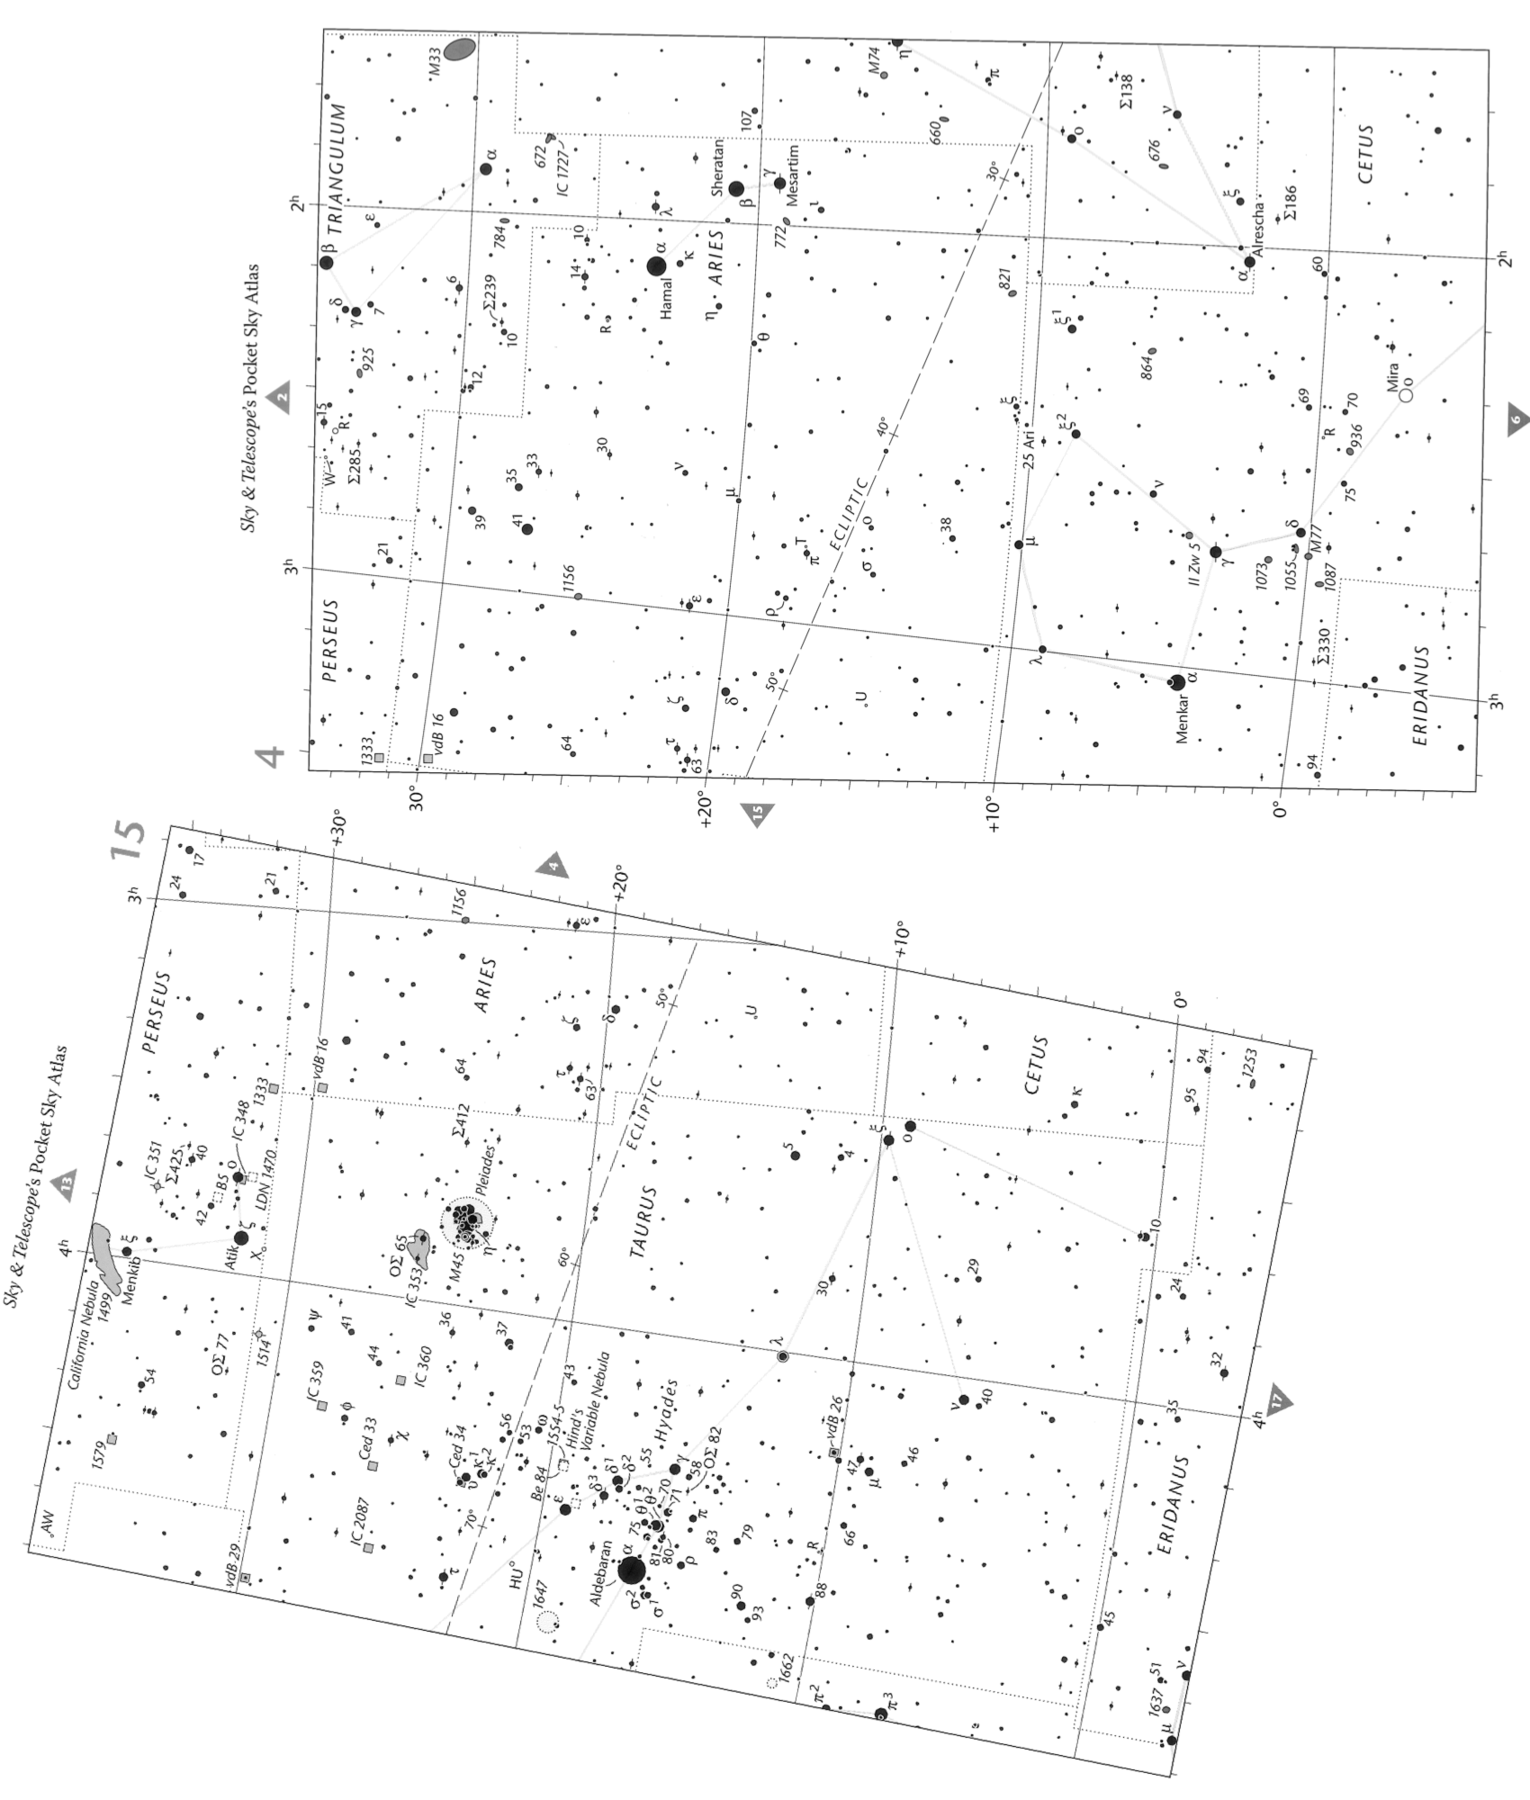
\includegraphics[width=7.5in]{mars-together.eps}

\clearpage

\noindent
{\bf Pay attention to the Moon}  

During lab, if we are outdoors, or sometime else in the week when the
weather is clear, look outside around 8pm and check if the Moon is
visible in the sky. Enter in the table below: (a) whether it is in the
East, West, or South; (b) what its phase is (full, new, crescent,
gibbous, and whether waxing or waning); and (c) guess what you will
find next week.

\begin{table}[h!]
\begin{tabular}{|c||c|c|c|}
\hline
{\bf Date} & {\bf Moon up at 8pm?} & {\bf Moon phase} & {\bf Guess for next
week} \cr
\hline
\hline
 & & & \cr
\hline
 & & & \cr
\hline
 & & & \cr
\hline
 & & & \cr
\hline
 & & & \cr
\hline
 & & & \cr
\hline
 & & & \cr
\hline
 & & & \cr
\hline
 & & & \cr
\hline
 & & & \cr
\hline
 & & & \cr
\hline
 & & & \cr
\hline
 & & & \cr
\hline
 & & & \cr
\hline
 & & & \cr
\hline
 & & & \cr
\hline
 & & & \cr
\hline
 & & & \cr
\hline
\end{tabular}
\end{table}


\end{document}
 
